\documentclass[11pt]{book}
\usepackage{hyperref}
\usepackage{colonequals}
\usepackage{amsfonts}
\usepackage{amssymb}
\usepackage{amsmath}
\usepackage[utf8]{inputenc}
\usepackage[T1]{fontenc}
\usepackage{float}
\usepackage{fixltx2e}
\usepackage[italian]{babel}
\usepackage{graphicx}

\newenvironment{sistema}%
{\left\lbrace\begin{array}{@{}l@{}}}%
{\end{array}\right.}


\title{Appunti di Ricerca Operativa}
\author{Fabio Viola}
\date{}

\setcounter{chapter}{6}

\begin{document}

\chapter{Problemi sui grafi}

\scriptsize
{\bf Slide}:
\href{http://www.or.deis.unibo.it/staff_pages/martello/Chapter7.zip}{Problems on Graphs}
\normalsize
\vspace{20pt}

\section{Introduzione}

La nascita della {\bf teoria dei grafi} si fa risalire al diciottesimo
secolo, periodo in cui {\bf Leonard Euler} formul\`o la domanda {\em
  esiste un cammino che parte da un punto e ritorna nello stesso punto
  attraversando tutti i ponti e rigorosamente una sola volta?}.

\begin{figure}[h!]
\centering
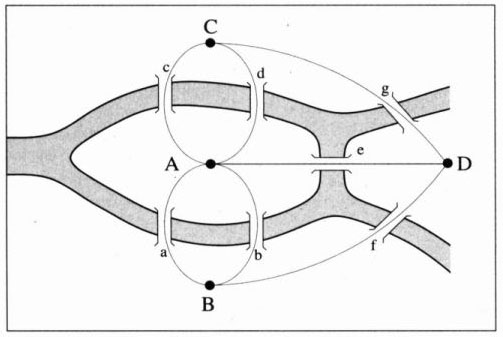
\includegraphics[width=0.5\textwidth]{images/cap7koni.jpg}
\caption{Problema di Konigsberg}
\label{cap7koni}
\end{figure}

Il problema (noto come {\em Problema di Konigsberg}) \`e il classico
esempio di problema modellabile tramite grafi, strutture composte da:

\begin{itemize}
\item vertici (nodi)
\item spigoli (collegamenti fra i nodi)
\end{itemize}


Il problema adattato all'ambito dei grafi diviene: {\em esiste un
  cammino chiuso che attraversa ogni spigolo esattamente una
  volta?}. Il problema viene rappresentato con il grafo in figura
\ref{cap7konig}.

\begin{figure}[h!]
  \centering
  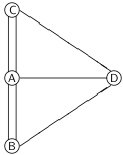
\includegraphics[width=0.3\textwidth]{images/cap7konig.png}
  \caption{Problema di Konigsberg}
  \label{cap7konig}
\end{figure}

Se questo cammino esiste, allora devono esserci per forza un nodo
entrante ed uno uscente in modo tale da consentire di entrare ed
uscire dal nodo (e dato che \`e consentito transitare anche pi\`u
volte dallo stesso nodo, purch\'e da spigoli diversi vi possono essere
pi\`u coppie). Traiamo dunque un importante risultato: il cammino
cercato pu\`o esistere soltanto se ogni vertice ha un numero pari di
spigoli che lo tocca. Dunque la soluzione al problema di Konigsberg
era che non esisteva il cammino.

\section{Terminologia}

Introduciamo la terminologia da utilizzare con i grafi. Un grafo si
dice {\bf semplice} o {\em multiplo}, a seconda che vi siano uno o
pi\`u spigoli fra due vertici. Noi considereremo soltanto grafi
semplici (a cui corrispondono un maggior numero di applicazioni
pratiche) e vedremo che quelli complessi molto spesso possono essere
trasformati in semplici.  I grafi possono poi essere {\em orientati}
o {\em non orientati} a seconda che gli spigoli possano essere
percorsi in una sola data direzione, e dunque $(v_i,v_k) \neq (v_i,
v_k)$, o in entrambe indifferentemente, cio\`e $(v_i,v_k) \equiv (v_i,
v_k)$. Nel primo caso ci riferiremo ai collegamenti col nome di {\em
  archi} (e li indicheremo con $a_i$), nel secondo li chiameremo {\em
  spigoli} (e li indicheremo con $e_i$). Gli elementi $a_i$ ed $e_i$
apparterranno rispettivamente agli insiemi $A$ ed $E$, mentre in ogni
caso i {\em vertici} apparterranno all'insieme $V$ e li indicheremo
con $v_i$. Gli archi e gli spigoli sono costituiti dalla coppia di
vertici che congiungono. Il grafo \`e dato dalla coppia $G=(V,E)$ nel
caso non orientato, dalla coppia $G=(V,A)$ nel caso orientato.

\begin{figure}[h!]
\centering
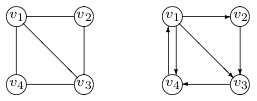
\includegraphics[width=0.7\textwidth]{images/cap7dirnondir.png}
\caption{Grafi non orientati e orientati}
\label{cap7dirnondir}
\end{figure}

Indichiamo con $\Gamma (v) = \{ v_j : (v, v_j) \in E \}$, l'insieme
dei nodi $v_j$ che possono essere raggiunti dal nodo $v$. Chiamiamo
{\bf grado} e lo indichiamo con $| \Gamma (v) |$ il numero di nodi
raggiungibili da $v$. Questo vale per i grafi non orientati. Per
quelli orientati si fa una distinzione fra $\Gamma^+$ e $\Gamma^-$
che sono rispettivamente l'insieme dei nodi $v_j$ raggiungibili da $v$
e l'insieme dei nodi $v_j$ da cui si pu\`o raggiungere
$v$. Riferendosi poi al grado si parler\`a nel primo caso di {\bf
  grado esterno}, nel secondo di {\bf grado interno}.

Chiamando $V'$ un sottoinsieme di vertici $v_i$ di $V$, si dice {\bf
  sottografo} di $G(V,A)$ o di $G(V,E)$ rispettivamente:

\begin{itemize}
\item $G' = (V',\`A)$ dove $\`A \subseteq \{(v_i,v_j) \in A : v_i, v_j \in V'\}$,
\item $G' = (V',\`E)$ dove $\`E \subseteq \{(v_i,v_j) \in E : v_i, v_j \in V'\}$.
\end{itemize}

Col termine {\bf grafo pesato} si intendono poi tutti quei grafi
(orientati o meno) i cui archi/spigoli hanno un {\bf costo}
associato.

Si definisce {\bf percorso} ({\em path}) una sequenza di archi/spigoli
senza ripetizioni di vertici. Un esempio di percorso (con riferimento
alla figura \ref{cap7dirnondir}) \`e $\{ v_1, v_4, v_3 \}$. Nel caso
di grafi orientati corrisponde al percorso che porta da $v_1$ a
$v_3$, mentre nel caso di grafi non orientati corrisponde sia al
percorso appena citato, sia a quello contrario. Definiamo {\bf
  circuito} o {\bf ciclo} un percorso che inizia e finisce sullo
stesso vertice.

Un grafo si dice {\bf connesso} (sia che esso sia orientato, sia che
non lo sia) se per ogni coppia di vertici $v_i$ e $v_j$ appartenenti a
$V$, esiste un percorso che porti dal primo al secondo.

\begin{figure}[h!]
  \centering
  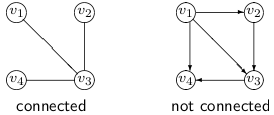
\includegraphics[width=0.7\textwidth]{images/cap7graficonnessi.png}
  \caption{Grafi connessi non connessi}
  \label{cap7graficonnessi}
\end{figure}

\section{Shortest Spanning Tree}

Il termine {\bf albero} indica un grafo con $n$ vertici che:

\begin{itemize}
\item \`e connesso e non contiene circuiti
\item \`e connesso e contiene $n-1$ spigoli
\item per ogni coppia $v_i$ e $v_j$ esiste un percorso dal primo al secondo.
\end{itemize}

Le tre condizioni sono equivalenti.

Dato $G=(V,E)$, un sottografo $G'=(V',\`E)$ che forma un albero \`e
detto {\bf spanning tree} ({\em ST}) di $G$. Una delle problematiche
affrontate dalla teoria dei grafi \`e quella che studia gli {\bf
  Shortest Spanning Tree} ({\em SST}), cio\`e dato un grafo $G=(V,E)$
pesato e connesso, trovare un {\em ST} $G' = (V,\`E)$ tale che
$\sum\limits_{e \in \`E w(e)}$ sia minimo. Assumeremo per semplicit\`a
che $w(e)$ (costo di uno spigolo) sia sempre maggiore o uguale a 0 per
ogni spigolo appartenente all'insieme $E$. Questi problemi trovano
numerose applicazioni nella vita reale, ad esempio per connettere
citt\`a con acquedotti al costo minore o per progettare circuiti
elettrici (vedere le leggi di Kirchhoff) solo per citarne alcuni.

{\bf Teorema:} dati $G=(V,E)$ ed un suo albero parziale (sottografo
che forma un albero) $(W,E')$ con $W \subset V$ ed $E' \subset E$, sia
$(\bar{u},\bar{v})$ il pi\`u corto degli spigoli $(u,v)$ tali che $u
\in W$, $v \in V \\ W$. Allora fra tutti gli spanning tree di $G$ che
contengono $E'$ ne esiste uno ottimo che contiene anche
$(\bar{u},\bar{v})$.

\vspace{11pt} $\square$ {\bf Dimostrazione}: sia $SST^*$ il pi\`u
corto $ST$ contenente $E'$, e supponiamo per assurdo che esso non
contenga $(\bar{u},\bar{v})$. In $SST^*$ deve esistere un cammino tra
$\bar{u}$ e $\bar{v}$ che conterr\`a almeno uno spigolo $(u,v)$ con $u
\in W$ e $v \in V \\ W$. Rimuovendo $(u,v)$ si otterrebbero due alberi
parziali ed aggiungendo $(\bar{u},\bar{v})$ si otterrebbe un nuovo
$ST$ pi\`u corto di $SST^*$ (contraddizione). $\blacksquare$
\vspace{11pt}

Segue dunque che se $(W,E')$ \`e ottimo (cio\`e \`e il pi\`u corto fra
gli alberi parziali di $G$ aventi per vertici $W$), allora ($W \cup \{
\bar{v}\}, E' \cup \{ (\bar{u}, \bar{v}) \}$) \`e ottimo. Abbiamo
quindi un semplicissimo algoritmo per $SST$:

\vspace{11pt}
\begin{center}
  \begin{tabular}{||l||}
    \hline\hline
    {\bf begin}\\
    \phantom{aa}$W := \{ w_1 \}, E' := \emptyset$ ({\bf commento:} albero parziale
    vuoto, quindi ottimo)\\
    \phantom{aa}{\bf while} $|W| < n$ {\bf do}:\\
    \phantom{aaaa}{\bf begin}\\
    \phantom{aaaaaa}determina $(\bar{u},\bar{v})$ come definiti dal teorema appena
    visto\\
    \phantom{aaaaaa}$W := W \cup \{ \bar{v} \}$, $E' := E' \cup \{
    (\bar{u},\bar{v})\}$\\
    \phantom{aaaa}{\bf end}\\
    {\bf end}\\
    \hline\hline
  \end{tabular}
\end{center}
\vspace{11pt}

Valutiamo lo sforzo computazionale richiesto dall'algoritmo in
funzione della dimensione del grafo. Il ciclo viene eseguito $n-1$
volte. Ad ogni iterazione, il numero di operazioni necessarie per
individuare $(\bar{u},\bar{v})$ \`e proporzionale ad $|E|$. Dato che
il grado di ogni vertice pu\`o avere un valore fino ad $n-1$, il
valore di $|E|$ sar\`a in generale proporzionale ad $n^2$ (sar\`a pari
a $n(n-1)/2$ nel caso peggiore). Complessivamente l'algoritmo richiede
dunque un tempo di calcolo proporzionale ad $n^3$, cio\`e la
complessit\`a dell'algoritmo \`e $O(n^3)$.

Vediamo come ottenere un algoritmo pi\`u efficiente. Associamo ad ogni
vertice $v$ non appartenente a $W$ un'{\bf etichetta} ({\em label}): 

\begin{center}
$b(v)$ = vertice di W cui \`e collegato con lo spigolo di costo minimo
\end{center}

In questo modo $(\bar{u},\bar{v})$ pu\`o essere trovato in un tempo
proporzionale a $n$. Ad ogni iterazione dovremo per\`o aggiornare i
valori $b(v)$ per i vertici $v \not\in W$. Osserviamo che ad ogni
iterazione, l'unica differenza rispetto all'iterazione precedente \`e
data dall'ingresso di $\bar{v}$ in $W$. Sar\`a quindi sufficiente
confrontare, per ogni vertice $v \not\in W$, il valore attuale del
nuovo spigolo possibile $w(v,\bar{v})$ ed eventualmente aggiornare
$b(v)$. Si ottiene cos\`i l'{\bf algoritmo di Prim}:

\vspace{11pt}
\begin{center}
  \begin{tabular}{||l||}
    \hline\hline
    {\bf procedure Shortest Spanning Tree}:\\
    {\bf begin}\\
    \phantom{aa}$W:=\{v_1\}; E':=\emptyset;$\\
    \phantom{aa}{\bf comment:} $b(v) = vertice \in W : w(v,b(v)) =
    \min\limits_{r \in W} \{ w(v,r) \}$;\\
    \phantom{aa}{\bf for each} $v \in V \textbackslash \{ v_1 \}$ {\bf do} $b(v)
    := v_1$;\\
    \phantom{aa}{\bf while} $|W| < n$ {\bf do}\\
    \phantom{aaaa}{\bf begin}\\
    \phantom{aaaaaa}trova $\bar{v} \in V \textbackslash W : w(\bar{v},b(\bar{v}))
    = \min\limits_{v \in V \textbackslash W} \{ w(v,b(v)) \}$;\\
    \phantom{aaaaaa}$W := W \cup \{ \bar{v} \}; E':= E' \cup \{
    (\bar{v},b(\bar{v}))\};$\\
    \phantom{aaaaaa}{\bf for each} $v \in V \textbackslash W$ {\bf do}\\
    \phantom{aaaaaaaa}{\bf if} $w(v,\bar{v}) < w(v,b(v))$ {\bf then}
    $b(v) := \bar{v}$\\
    \phantom{aaaa}{\bf end}\\
    {\bf end.}\\
    \hline\hline
  \end{tabular}
\end{center}
\vspace{11pt}

Anche il nuovo algoritmo richiede $n-1$ iterazioni, ma ad ogni
iterazione, il numero di operazioni \`e proporzionale a $|V
\textbackslash W|$, ossia ad $n$ nel caso peggiore. In totale quindi
l'algoritmo di Prim risolve SST in tempo $O(n^2)$. 

\vspace{11pt} $\blacktriangleright$ {\bf Esempio}: consideriamo il
primo grafo in figura \ref{cap7fig73}. I grafi successivi mostrano
l'albero parziale alle varie iterazioni. Il valore $b(v)$ \`e mostrato
accanto a $v$, tra parentesi quadre. $\blacktriangleleft$
\vspace{11pt}

\begin{figure}[h!]
  \centering
  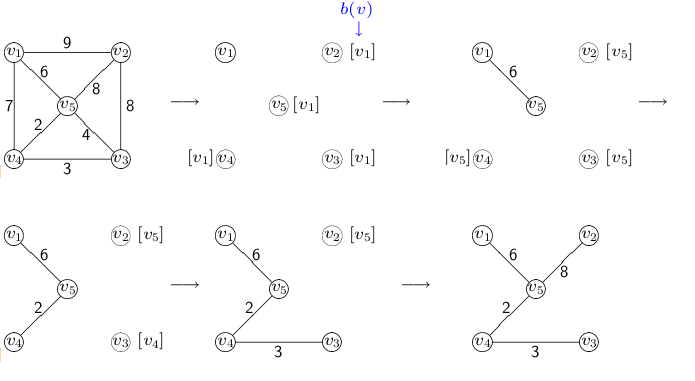
\includegraphics[width=\textwidth]{images/cap7fig73.png}
  \caption{esempio dell'algoritmo di Prim}
  \label{cap7fig73}
\end{figure}

\section{Rappresentazione dei grafi}

Per rappresentare i grafi si possono utilizzare diverse strutture
dati. Vedremo le principali. I vertici $v_1, \dots, v_n$, vengono
rappresentati dagli interi $1, \dots, n$. Per quanto riguarda la
rappresentazione degli archi/spigoli, la scelta dipende dalla {\bf
  densit\`a}. Un grafo di $n$ vertici ed $m$ archi si dice {\bf denso}
se $m \approx n^2$, mentre viene detto {\bf sparso} se $m \ll
n^2$. Informalmente si dice che ha {\em molti} o {\em pochi}
archi/spigoli.

\subsection{Grafi densi}

Se il grafo non \`e pesato si usa la {\bf matrice di adiacenza} $A$
quadrata di ordine $n$ in cui abbiamo tante righe e tante colonne
quanti sono i vertici. La cella $ij$ che incrocia la riga relativa al
vertice $i$ e la colonna relativa al vertice $j$ vale 1 se esiste un
arco/spigolo $(v_i, v_j)$ che unisce i due vertici, altrimenti vale 0.

\begin{center}
$a_{ij} = 
\begin{sistema}
1\phantom{aaa} se (v_i, v_j) \in A\phantom{aa}[\in E];\\
0\phantom{aaa} altrimenti
\end{sistema}
$
\end{center}

Se il grafo \`e pesato si usa la {\bf matrice dei pesi} $W$, anche
questa quadrata di ordine $n$. In questa matrice anzich\'e avere 0
quando non esiste un arco, avremo $+\infty$ (se il problema \`e di
minimizzazione) o $-\infty$ (se il problema \`e di
massimizzazione). Nelle celle dove avremmo posto 1, poniamo ora il
peso del collegamento. 

\begin{center}
$w_{ij} = 
\begin{sistema}
w(v_i,v_j)\phantom{aaa} se (v_i, v_j) \in A\phantom{aa}[\in E];\\
\pm\infty \phantom{aaa} altrimenti
\end{sistema}
$
\end{center}

In figura \ref{cap7figura74} possiamo notare come si costruiscano la
matrice di adiacenza e la matrice dei pesi.

\begin{figure}[h!]
  \centering
  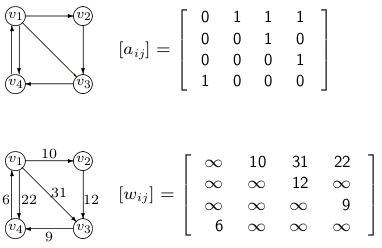
\includegraphics[width=0.7\textwidth]{images/cap7figura74.png}
  \caption{Esempio}
  \label{cap7figura74}
\end{figure}

Per grafi non orientati le matrici di adiacenza e dei pesi sono
simmetriche rispetto alla diagonale principale. Si possono quindi
eventualmente usare delle strutture dati apposite per aumentare
l'efficienza.

\subsection{Grafi sparsi}

Per i grafi sparsi si memorizzano soltanto gli archi esistenti
mediante la cosiddetta {\bf forward star} dei nodi. La forward star
\`e formata da:

\begin{itemize}

\item un vettore {\em u} di {\em m} elementi (cio\`e tanti elementi
  quanti sono gli archi). Questo vettore si costruisce partendo dal
  primo vertice, andando verso l'ultimo prendendo per ogni vertice i
  destinatari degli archi che partono da esso. Ad esempio per il grafo
  in figura \ref{cap7figura74} partiamo dal vertice 1 e troviamo tre
  archi diretti verso 2, 3 e 4. Poi prendiamo il secondo vertice e
  abbiamo un arco diretto verso 3 e inseriamo tale valore nella
  lista. Passiamo al nodo 3 e troviamo un arco uscente verso il
  vertice 4 dunque inseriamo 4 nella lista, poi per l'ultimo vertice
  abbiamo un arco diretto al vertice 1, quindi inseriremo 1 e otterremo il
  vettore $w' = (2, 3, 4, 3, 4, 1)$.

\item un vettore {\em w} che esiste \underline{solo se il grafo \`e
  pesato} di {\em m} elementi (cio\`e tanti elementi quanti sono gli
  archi). Questo vettore si costruisce partendo dal primo vertice,
  andando verso l'ultimo prendendo per ogni vertice il costo degli
  archi che partono da esso. Ad esempio per il grafo in figura
  \ref{cap7figura74} partiamo dal vertice 1 e troviamo tre archi di
  peso 10, 31 e 22. Poi prendiamo il secondo vertice e abbiamo un arco
  di peso 12 e lo inseriamo nella lista. Passiamo al nodo 3 e troviamo
  un arco uscente di peso 9 dunque inseriamo 9 nella lista, poi per
  l'ultimo vertice abbiamo un arco di peso 6, quindi inseriremo 6 e
  otterremo il vettore $w' = (10, 31, 22, 12, 9, 6)$.
  
\item un vettore {\em p} di $n+1$ elementi (cio\`e uno pi\`u dei
  vertici).  Gli elementi di {\em p} sono dei puntatori agli elementi
  di {\em u} e {\em w}. Le informazioni del vertice di partenza 1 sono
  inserite nei vettori {\em u} e {\em w} a partire dalla posizione 1,
  pertanto il puntatore $p_1$ avr\`a valore 1, cio\`e punter\`a alla
  posizione 1 dei vettori {\em u} e {\em w}. Le informazioni dei
  successivi nodi genericamente indicati con $p_i$ da quale posizione
  di {\em u} (e {\em w}) partono? Bene, a quella posizione punteranno
  gli elementi di $p$. L'ultimo elemento del vettore $p$, cio\`e
  $p_{n+1}$ avr\`a valore $m+1$.

  Facendo riferimento all'esempio: il primo elemento ha sempre come
  puntatore 1; le informazioni nel vettore {\em u} relative al primo
  nodo sono le prime tre, dunque le informazioni prese dal secondo
  elemento sono inserite in posizione 4, pertanto avremo in $p_2$ un
  puntatore alla posizione 4. Le informazioni degli archi che partono
  dal nodo 3 sono contenute nelle posizioni a partire dalla 5 (in
  realt\`a occupano una sola posizione, ma questo ci intereser\`a al
  prossimo giro) dunque inseriamo 5 nel vettore. Per la considerazione
  fatta poc'anzi le informazioni degli archi che partono dal vettore 4
  iniziano dalla posizione 6 pertanto inseriamo nella lista l'elemento
  6. L'ultimo elemento, $p_{n+1} = p_{5}$ varr\`a $m+1 = 7$ per
  definizione. Il vettore costruito \`e pertanto $p' = (1,4,5,6,7)$.

\end{itemize}

La forward star, come abbiamo visto, consente di accedere facilmente
agli archi/spigoli uscenti da un vertice, ma non a quelli entranti. Se
si vuole accedere rapidamente anche ad essi si deve accoppiare alla
precedente la struttura {\bf reverse star}:

\begin{itemize}

\item un vettore {\em e} di {\em m} elementi in cui per ogni vertice,
  partendo dal primo e andando verso l'ultimo, inseriamo il vertice da
  cui ci siamo arrivati. Ha ovviamente {\em m} elementi. Nel caso in
  esame partiamo dal nodo 1: ad esso si arriva dal vertice 4 dunque
  inseriamo 4 come primo elemento di {\em e}. Poi passiamo al vertice
  2: questo ha come arco entrante solo quello partente da 1, dunque
  inseriamo 1 nella lista. Il nodo 3 ha come archi entranti quello che
  parte da 1 e quello che parte da 2, dunque inseriamo 1 e 2 nella
  lista. Il nodo 4 ha come nodo entrante solo quello che parte da 3,
  dunque inseriamo 3 nella lista. Il vettore \`e $e' = (4,1,1,2,1,3)$;
  
\item un vettore $\bar{w}$ costruito come $w$ ma prendendo i nodi
  entranti anzich\'e quelli uscenti. Ha ovviamente {\em m}
  elementi. Il vettore in questo caso \`e $\bar{w} = 6, 10, 31, 12,
  22, 9$. 

\item un vettore {\em q} di {\em n+1} elementi costruito con le stesse
  modalit\`a di {\em p}. In questo caso il vettore \`e: $q' = (1, 2,
  3, 5, 7)$.

\end{itemize}

Per i grafi non orientati non ha interesse la seconda struttura in
quanto non vi \`e alcuna distinzione fra spigoli entranti ed uscenti.


\section{Cammini minimi}


Dati due vertici $v_i$ e $v_j$, il {\bf cammino minimo} da $v_i$ a
$v_j$ \`e quello la cui somma dei pesi degli archi che lo compongono
\`e minima. \`E chiaro dunque come tali problemi assumano una
particolare importanza: facile immaginare applicazioni nel campo dei
trasporti, ma tali problemi son frequenti anche nelle comunicazioni,
nel layout di impianti industriali, nella robotica, ecc\dots


A seconda dell'applicazione possiamo essere interessati a trovare:


\begin{itemize}
\item il cammino minimo fra due vertici;
\item i cammini minimi da un vertice a tutti gli altri;
\item i cammini minimi fra tutte le coppie di vertici.
\end{itemize}


Quello fondamentale al momento \`e il secondo. Considereremo dunque il
problema {\bf Shortest Path Problem} ({\em SPP}):


\begin{quote}
Dato un grafo pesato $G=(V,A)$ e dato un vertice $s \in V$ (sorgente),
trovare per ogni $v \in V \textbackslash \{s\}$ il cammino pi\`u breve
da {\em s} a {\em v}.
\end{quote}


A questo proposito possiamo introdurre una {\bf propriet\`a}: se il
cammino minimo da $v_i$ a $v_k$ passa per $v_j$, esso \`e formato dal
cammino minimo da $v_i$ a $v_j$ e dal cammino minimo da $v_i$ a $v_k$


\vspace{11pt}
$\square$ {\bf Dimostrazione}: se esistesse un cammino pi\`u breve da
$v_i$ a $v_j$ (o da $v_j$ a $v_k$) esso verrebbe usato anche nel
cammino minimo da $v_i$ a $v_k$. $\blacksquare$
\vspace{11pt}


Definiamo {\bf arborescenza} un grafo orientato privo di circuiti in
cui un vertice (che chiamiamo {\bf radice}) ha semigrado entrante
nullo e tutti gli altri vertici hanno semigrado entrante pari a 1. (In
altre parole il nodo radice non ha genitori, cio\`e non ha archi
entranti, e gli altri nodi hanno un solo arco entrante).


Con riferimento alla figura \ref{cap7figura74} possiamo costruire
un'arborescenza con radice in $v_1$ e insieme di archi $\{(v_1, v_2),
(v_1, v_3), (v_1, v_4)\}$ o ancora, sempre con radice in $v_1$
prendendo l'insieme di archi $\{(v_1, v_2), (v_2, v_3), (v_1, v_4)\}$.


Un insieme di cammini minimi da $s$ agli altri vertici forma
un'arborescenza con radice in $s$.

\vspace{11pt}
$\square$ {\bf Dimostrazione}: ogni vertice tranne {\em s} deve avere
almeno un arco entrante. Se un vertice {\em v} avesse due archi
entranti si potrebbe eliminare quello appartenente al cammino pi\`u
lungo da {\em s} a {\em v}.
$\blacksquare$
\vspace{11pt}


Per i problemi di cammino minimo \`e importante considerare anche
grafi i cui archi/spigoli possano avere pesi negativi. Considereremo
separatamente i casi di grafi con pesi {\underline non} negativi da
quelli con pesi negativi.


\subsection{Grafi con pesi non negativi}

Il metodo principale per problemi di cammini minimi \`e l'{\bf
  Algoritmo di Dijkstra} che estende progressivamente un'arborescenza
parziale con radice in {\em s}, contenente vertici gi\`a raggiunti da
cammini minimi. 

Sia {\em s} l'insieme dei vertici che appartengono all'arborescenza
parziale (inizialmente $S = \{s\}$). Inseriremo nel grafo a fianco ad
ogni vertice il costo per raggiungere il vertice con un arco che parte
da $s$.

\begin{figure}[H]
  \centering
  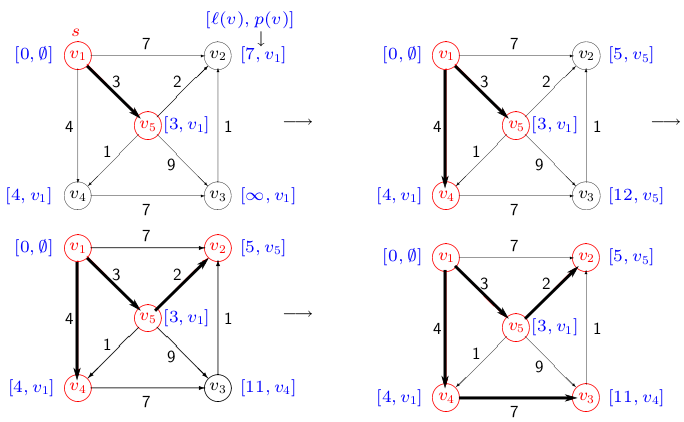
\includegraphics[width=\textwidth]{images/cap7fig75.png}
  \caption{Esempio di applicazione dell'algoritmo di Dijkstra}
  \label{cap7fig75}
\end{figure}


Con riferimento al grafo di figura \ref{cap7figura75} l'insieme $S$
sar\`a all'inizio formato solo da $v_1$. Per raggiungere $v_2$ con un
arco che parte da $v_1$ il costo \`e 7, il nodo da cui ci siamo
arrivati \`e appunto $v_1$, pertanto metteremo accanto al vertice
$v_2$ la dicitura $[7,v_1]$. Faremo lo stesso per gli altri vertici.


Ad ogni iterazione scegliamo un arco fra quelli che vanno da un
vertice di {\em S} ad un vertice $\bar{v}$ non di {\em S}. In
particolare sceglieremo il vertice il cui costo di percorso \`e minimo
e lo inseriamo in $S$. A questo punto si aggiornano le etichette dei
vertici che i cui costi, passando dal nodo in esame,
diminuirebbero. Con riferimento all'esempio prendiamo nella prima
iterazione il vertice $v_5$ in quanto il costo per arrivare in quel
vertice \`e il minore. Aggiorniamo il costo per arrivare al vertice
$v_2$ che scende da 7 a 5, dunque la sua etichetta diviene $[5,
  v_5]$. Aggiorniamo anche l'etichetta di $v_3$ che passa da $[\infty,
  v_1]$ a $[12, v_5]$. Continueremo ad iterare finch\'e non terminiamo
i vertici.


L'algoritmo \`e dunque:

\small
\vspace{11pt}
\begin{center}
\begin{tabular}{||l||}
\hline\hline
{\bf procedure Shortest Paths}:\\
{\bf begin}\\
\phantom{ss}$S:= \{s\}; \mathit{l}(s) := 0; p(s) := \emptyset;$\\
\phantom{ss}{\bf commento:} $S$ \`e l'insieme dei vertici raggiunti con cammini minimi;\\
\phantom{ss}{\bf commento:} $\mathit{l}(v)$ \`e la lungh del cammino min da $s$ a $v$ passante per vertici $\in S$;\\
\phantom{ss}{\bf commento:} $p(v)$ \`e il predecessore di $v$ nel cammino lungo $\mathit{l}(v)$;\\
\phantom{ss}{\bf for each} $v \in V \textbackslash \{s\}$ {\bf do}\\
\phantom{ssss}{\bf begin}\\
\phantom{ssssss}$\mathit{l}(v) := w(s,v)$;\\
\phantom{ssssss}$p(v) := s$\\;
\phantom{ssss}{\bf end};\\
\phantom{ss}{\bf while} $S \neq V$ {\bf do}\\
\phantom{ssss}{\bf begin}\\
\phantom{ssssss}trova $\bar{v} \in V \textbackslash S$ : $\mathit{l}(\bar{v}) = \min\limits_{v \in V \textbackslash \phantom{ss}S}\{\mathit{l}(v)\}$;\\
\phantom{ssssss}$S := S \cup \{\bar{v}\}$\\
\phantom{ssssss}{\bf for each} $v \in V \textbackslash S$ {\bf do}\\
\phantom{ssssssss}{\bf if} $\mathit{l}(\bar{v}) + w(\bar{v},v) < \mathit{l}(v)$ {\bf then}\\
\phantom{ssssssssss}{\bf begin}\\
\phantom{ssssssssssss}$\mathit{l}(v) := \mathit{l}(\bar{v}) + w(\bar{v},v)$;\\
\phantom{ssssssssssss}$p{v} := \bar{v}$\\
\phantom{ssssssssss}{\bf end}\\
\phantom{ssss}{\bf end}\\
{\bf end.}\\
\hline\hline
\end{tabular}
\end{center}
\vspace{11pt}
\normalsize

Nell'arborescenza abbiamo inserito il vertice $\bar{v}$ (e quindi
l'arco $(p(\bar{v}),\bar{v})$) sulla base del seguente teorema:


{\bf Teorema}: se $\mathit{l}(\bar{v}) = \min\limits_{v \in V
  \textbackslash S}\{ \mathit{l}(v) \}$, il cammino da {\em s} a
$\bar{v}$ \`e lungo $\mathit(\bar{v})$.

\vspace{11pt}
$\square$ {\bf Dimostrazione}: dimostriamo che qualunque cammino {\em
  P} da {\em s} a $\bar{v}$ \`e lungo almeno
$\mathit{l}(\bar{v})$. Esistono due possibilit\`a:

\begin{itemize}
\item se {\em P} passa solo per vertici di {\em S}, la tesi \`e vera
  per definizione di $\mathit{l}$;
\item altrimenti, sia {\em h} il primo vertice $\not \in S$ che si
  incontra in {\em P}. {\em P} \`e dunque formato dalla concatenazione
  di un cammino da {\em s} ad {\em h} (lungo almeno $\mathit{l}(h)
  \geq \mathit{l}({\bar{v}})$) e un cammino da {\em h} a $\bar{v}$ di
  lunghezza $\geq 0$.$\blacksquare$
\end{itemize}
\vspace{11pt}

Questo algoritmo esegue {\em n-1} iterazioni del ciclo {\bf while}. Ad
ogni iterazione il numero di operazioni \`e proporzionale a $|V
\textbackslash S|$. Complessivametne l'algoritmo ha dunque
complessit\`a $O(n^2)$.


Abbiamo preso in esame il problema numero due di quell'elenco visto
all'inizio della sezione. Cosa dobbiamo fare se vogliamo solo il
cammino minimo da $s \in V$ a $t \in V$ (cio\`e quando vogliamo
risolvere il problema uno)? Non esiste un metodo migliore
dell'algoritmo di Dijkstra, quindi la soluzione \`e quella di fermarsi
non appena $t \in S$. In termini di algoritmo dovremmo sostiture
\textquotedblleft {\bf while} $S \neq V$ {\bf do}\textquotedblright
con \textquotedblleft {\bf while} $t \not\in S$ \textquotedblright. La
complessit\`a dell'algoritmo resta la medesima.


Volendo invece risolvere il terzo problema si applica {\em n} volte la
procedura, una volta per ogni possibile sorgente. L'algoritmo diviene
dunque \textquotedblleft {\bf for each} $s \in V$ {\bf do call
  Shortest Paths}. La complessit\`a diventa ovviamente $O(n^3)$.


\subsection{Grafi con pesi negativi}


La prima osservazione da fare \`e che il grafo {\underline {\bf non}}
deve contenere {\bf circuiti di lunghezza negativa}, cio\`e cammini
chiusi tali per cui la somma dei costi degli archi/spigoli sia
negativa. In tali casi il problema perde significato perch\'e
immaginando di stressare il problema effettuando infinite percorrenze
di tale circuito, otterremmo un cammino non semplice di lunghezza
$-\infty$! Prendiamo dunque in esame grafi sprovvisti di circuiti
negativi. In tali situazioni esiste una versione modificata
dell'algoritmo di Dijkstra (che per\`o ha complessit\`a $O(n^3)$) per
trovare l'arborescenza dei cammini minimi con radice in $s$.


\`E da sottolineare che per\`s in questo caso si preferisce usare un
altro metodo basato sulla stessa idea, noto come algoritmo di Floyd e
Warshall che nello stesso tempo trova le lunghezze dei cammini fra
tutte le coppie di vertici!


\subsection{Problema del cammino pi\`u lungo}


Questo problema, noto come {\bf Longest Path Problem} ({\em LPP}), \`e
enormemente pi\`u complesso. Non esiste un modo per adattare gli
algoritmi per il cammino minimo visti poco fa. Si procede dunque
utilizzando degli algoritmi branch and bound con conseguente
costruzione di un albero decisionale. Tale metodo pu\`o degenerare in
un'{\bf enumerazione completa} e ci\`o porterebbe ad una complessit\`a
di $O((n-1)!)$.




\section{Problema del flusso massimo}


In molte applicazioni, i grafi rappresentano un sistema di condotte
lungo le quali pu\`o fluire un materiale. Ogni arco avr\`a una
limitazione sulla massima quantit\`a di materiale che pu\`o
attraversarlo per unit\`a di tempo. Non avremo dunque dei grafi
pesati, ma dei grafi sui cui archi troveremo le {\bf capacit\`a} $q$
(che assumiamo intere). In particolare $q_{ij}$ \`e la capacit\`a
dell'arco $(v_i, v_j)$.


I problemi del flusso massimo sono utili ad esempio per studiare il
traffico in un sistema di strade, o per applicazioni riguardanti
oleodotti o gasdotti o ancora reti elettriche.


Il {\bf problema del flusso massimo} ({\em MFP}) \`e il seguente:


\begin{quote}
Dato $G=(V,A)$, con capacit\`a associate agli archi, e dati due
vertici $s, t \in V$ (rispettivamente detti sorgente e terminale),
inviare il massimo flusso possibile da $s$ a $t$.
\end{quote}


Oltre ad individuare il flusso massimo, in alcuni casi potremmo anche
essere interessati a trovare gli eventuali colli di bottiglia per
poter in futuro aumentare la capacit\`a del sistema.


Per affrontare il problema in questione dobbiamo introdurre il
concetto di flusso. Un insieme di valori $\xi_{ij}$ (flusso da $v_i$
a $v_j$) per $i,j=1,\dots,n$ viene detto {\bf flusso ammissibile} di
valore {\em z} da {\em s} a {\em t} se:


\begin{itemize}
\item $0 \leq \xi_{ij} \leq q_{ij}\phantom{aaaaa}\forall (v_i, v_j) \in A$
\item $\sum\limits_{v_j \in \Gamma^+ (v_i)}\xi_{ij} - \sum\limits_{v_k \in \Gamma^+ (v_i)}\xi_{ki} = \begin{sistema}
+z\phantom{aaa}v_i=s\\
-z\phantom{aaa}v_i=t, \forall v_i \in V\\
0\phantom{aaaa}altrimenti
\end{sistema}$
\end{itemize}


La seconda equazione \`e nota come {\bf equazione di conservazione del
  flusso} ed esprime il vincolo che, per ogni vertice, esclusi la
sorgente ed il terminale, il flusso totale entrante sia uguale al
flusso totale uscente.


Definiamo {\bf Taglio {\em s-t}} una partizione dell'insieme $V$ in
due insiemi $V_1$ e $V_2$ tali che $s \in V_1$ e $t \in V_2$. Si dice
{\bf valore del taglio} la quantit\`a:
\begin{center}
$\sum\limits_{(v_i,v_j) : v_i \in V_1, v_j \in V_2} q_{ij}$
\end{center}
cio\`e la sommatoria di tutte le capacit\`a degli archi che partono da
vertici dell'insieme $S_1$ e arrivano in vertici dell'insieme $S_2$.


A cosa ci serve la definizione di taglio? Ce lo dice il {\bf teorema
  fondamentale del flusso}: il valore $z$ del massimo flusso da $s$ a
$t$ \`e uguale al minimo valore di un taglio $s-t$.

\vspace{11pt} $\square$ {\bf Dimostrazione}: dato un taglio qualunque,
tutto il flusso da {\em s} a {\em t} deve attraversarlo, per cui non
pu\`o esserci nessuna soluzione di valore maggiore di
$\sum\limits_{(v_i,v_j) : v_i \in V_1, v_j \in V_2} q_{ij}$.

Questo vale ovviamente anche per il taglio di valore
minimo. Mostreremo pertanto che esiste un flusso di tale valore
mediante una {\bf dimostrazione costruttiva}, ossia dando un algoritmo
che trova il flusso richiesto.

Dato un flusso ammissibile $\xi_{ij}$ proponiamoci di trovare un
taglio qualunque mediante la seguente semplicissima procedura:

\vspace{11pt}
\begin{center}
  \begin{tabular}{||l||}
    \hline\hline
    $V_1 \colonequals \{ s \};$\\
    {\bf while} $\exists v_i \in V_1$ e $v_j \not\in V_1 : \xi_{ij} <
    q_{ij}$ o $\xi_{ji} > 0$ {\bf do} $V_1 \colonequals V_1 \cup \{ v_k\}$.\\
    \hline\hline
  \end{tabular}
\end{center}
\vspace{11pt}

La procedura pu\`o terminare avendo inserito il vertice terminale {\em
  t} in $V_1$, oppure senza averlo inserito. Esaminiamo le
implicazioni nei due casi:

\begin{itemize}
  
\item {\bf Caso 1: $t \in V_1$}, non \`e stato trovato un taglio {\em
  s-t}. Sappiamo allora che esiste una sequenza di archi che collega
  {\em s} a {\em t}. Tale sequenza non \`e un cammino in quanto la
  procedura aggiunge archi in entrambe le direzioni (vedere nella
  figura \ref{cap7fig77} in alto) e viene detta {\bf catena
    aumentante}. Chiameremo {\em archi avanti} quelli orientati da
  {\em s} verso {\em t} ed {\em archi indietro} gli altri. Il termine
  {\em aumentante} deriva dal fatto che mediante essa \`e possibile
  aumentare il flusso attuale $\xi$. Osserviamo infatti che per
  costruzione $\xi$ soddisfa:

  \begin{itemize}
  \item $\xi_{ij} < q_{ij}$ per ogni arco avanti $(v_i,v_j)$;
  \item $\xi_{kl} > 0$ per ogni arco indietro $(v_k,v_l)$.
  \end{itemize}

  \begin{figure}[H]
    \centering
    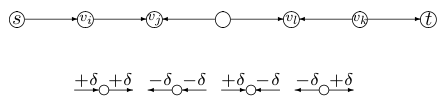
\includegraphics[width=0.8\textwidth]{images/cap7fig77.png}
    \caption{Catena aumentante da {\em s} a {\em t} e possibili
      incrementi del flusso}
    \label{cap7fig77}
  \end{figure}

  Definiamo allora:

  \begin{itemize}
  \item $\delta_1 = \min \{(q_{ij} - \xi_{ij}): (v_i,v_j) \text{ \`e
    avanti}\}$;
  \item $\delta_2 = \min \{ \xi_{kl}: (v_k,v_l) \text{ \`e indietro}
    \}$;
  \item $\delta = \min (\delta_1,\delta_2)$.
  \end{itemize}

  Aggiungendo $\delta$ al flusso di ogni arco avanti e sottraendolo
  dal flusso di ogni arco indietro si ottiene un nuovo flusso che
  soddisfa:

  \begin{itemize}
  \item $0 \leq \xi_{ij} \leq q_{ij}\phantom{aaaaa}\forall (v_i, v_j)
    \in A$ per definizione di $\delta$;
  \item $\sum\limits_{v_j \in \Gamma^+ (v_i)}\xi_{ij} - \sum\limits_{v_k \in \Gamma^+ (v_i)}\xi_{ki} = \begin{sistema}
    +z\phantom{aaa}v_i=s\\
    -z\phantom{aaa}v_i=t, \forall v_i \in V\\
    0\phantom{aaaa}altrimenti
  \end{sistema}$ come si verifica facilmente nei quattro casi mostrati
    in figura \ref{cap7fig77}.
  \end{itemize}

  Si ottiene quindi un nuovo flusso ammissibile $\xi$ con valore
  aumentato di $\delta$ unit\`a al quale si pu\`o riapplicare la
  seconda procedura, e cos\`i via, iterando fino a quando si termina
  nella seconda situazione.

\item {\bf Caso 2: $t \not\in V_1$}, \`e stato trovato un taglio {\em
  s-t}. Ci\`o implica che nessuna delle due condizioni di controllo
  del ciclo {\em while} \`e soddisfatta, ossia:

  \begin{itemize}
  \item $\xi_{ij} = q_{ij} \forall (v_i,v_j) : v_i \in V_1, v_j \in
    V_2$;
  \item $\xi_{ij} = 0 \forall (v_k,v_l) : v_k \in V_2, v_l \in V_1$.
  \end{itemize}

  Quindi il valore attuale del flusso che attraversa il taglio trovato
  \`e pari a:

  \begin{center}
 $\sum\limits_{(v_i,v_j) : v_i \in V_1, v_j \in V_2} q_{ij}$
  \end{center}
  
 e quindi \`e ottimo. Si osservi infine che il taglio individua il
 collo di bottiglia, dato dagli archi saturi che lo attraversano da
 $V_1$ verso $V_2$.$\blacksquare$

\end{itemize}
\vspace{11pt}


Dalla dimostrazione del teorema deriva un metodo per la soluzione del
problema del flusso massimo: si inizia con un flusso ammissibile (ad
esempio $\xi_{ij} = 0 \forall (v_i,v_j) \in A$) e lo si incrementa
iterativamente mediante catene aumentanti. Quando non ci sono pi\`u
catene aumentanti il flusso \`e massimo. Per trovare le catene
aumentanti utilizziamo un algoritmo di etichettamento dei vertici. In
particolare associamo un'etichetta ad ogni vertice di $V_1$ e poi
cercheremo di aggiungere vertici a $V_1$.


Un vertice pu\`o essere:
\begin{itemize}
\item non etichettato;
\item etichettato e non esplorato;
\item etichettato ed esplorato.
\end{itemize}


L'etichetta pu\`o essere:
\begin{itemize}
\item $[+v_k, \delta]$: se $\xi_{ki}$ pu\`o essere aumentato
\item $[-v_k, \delta]$: se $\xi_{ik}$ pu\`o essere diminuito
\end{itemize}
dove $\delta$ \`e il massimo flusso addizionale che si pu\`o mandare da $s$ a $v_i$.


\vspace{11pt} $\blacktriangleright$ {\bf Esempio}: consideriamo il
grafo in figura \ref{cap7figura78} e vediamo come svolgere l'algoritmo.

\begin{figure}[h!]
  \centering
  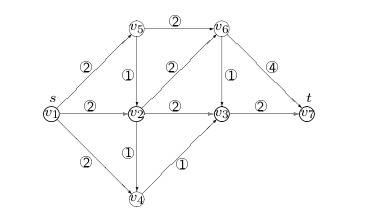
\includegraphics[width=0.77\textwidth]{images/cap7figura78.png}
  \caption{Grafo iniziale}
  \label{cap7figura78}
\end{figure}

\begin{itemize}

\item {\bf Inizializzazione}: pongo $\xi_{ij} = 0$ (cio\`e inizializzo
  a 0 il flusso sull'arco $(v_i,v_j)$) per ogni $i$ e $j$. E imposto
  la variabile {\em opt} a {\em false} (in quanto all'inizio ancora
  non abbiamo l'ottimo). Etichetto il vertice di partenza $v_1$ con
  $[+s, +\infty]$.
  
\item {\bf Prima iterazione del repeat (prima iterazione del while)}:
  prendo il primo vertice etichettato ma non ancora esplorato (dunque
  $v_1$). Per ogni vertice $v_j \in \Gamma^+$, cio\`e uscente da $v_i$
  (e in questo caso parliamo di $v_2$, $v_4$, $v_5$) tale per cui
  $\xi_{ij} < q_{ij}$ (cio\`e tale per cui il flusso \`e minore del
  massimo flusso trasportabile) etichettiamo il vertice $v_j$ con
  $[+v_i, \min(\delta(v_i), q_{ij}-\xi_{ij}]$. Nella fattispecie
  avremo:

  \begin{itemize}
  \item per il vertice $v_2$ vale $\xi_{ij} < q_{ij}$ in quanto $0 <
    2$, pertanto etichettiamo il vertice con $[+v_1, 2]$;
  \item stesso discorso (e casualmente anche con gli stessi valori)
    vale per $v_4$, dunque etichettiamo $v_4$ con $[+v_1, 2]$;
  \item ancora una volta stessi valori per $v_5$, dunque $[+v_1, 2]$.
  \end{itemize}

  Non avendo archi entranti non c'\`e altro da fare per $v_1$. Lo
  marchiamo come esplorato (nel grafico aggiungiamo un pallino nero).

\item {\bf Seconda iterazione del repeat (prima iterazione del
  while)}: prendiamo un vertice fra quelli etichettati ma non
  esplorati. Abbiamo a disposizione $v_2$, $v_4$ e $v_5$. Prendiamo il
  primo, $v_2$ (consideriamo sempre il primo in ordine crescente).

  \begin{itemize} 
  \item {\bf Archi uscenti}: quelli verso $v_3$ e $v_6$. Con lo stesso
    procedimento visto nella precedente iterazione etichettiamo $v_3$
    con $[+v_2, 2]$ e $v_6$ con $[+v_2, 2]$.

  \item {\bf Archi entranti}: quelli provenienti da $v_1$, $v_4$ e
    $v_5$. Adesso abbiamo per la prima volta a che fare con degli
    archi entranti. Vediamo come comportarci: per ogni vertice $v_j$
    proveniente da un arco entrante e tale per cui il flusso sia
    maggiore di 0 etichettiamo il vertice $v_j$ con $[v_j,
      \min(\delta(v_i),\xi_{ji})]$. In questo caso pur avendo
    individuato dei vertici $v_j$, per essi non vale $\xi_{ji} > 0$
    dunque non facciamo nulla. 
  \end{itemize} 

  Marchiamo $v_2$ come esplorato.

\item {\bf Terza iterazione del repeat (prima iterazione del while)}:
  a questo punto i vertici etichettati non esplorati sono $v_3$,
  $v_4$, $v_5$. Prendiamo $v_3$. L'unico arco uscente \`e diretto
  verso $v_7$ che non \`e etichettato, pertanto lo etichettiamo con
  $[+v_3, 2]$. Gli archi entranti provengono da $v_2$, $v_4$ e
  $v_6$. Tali vertici, essendo gi\`a stati etichettati non si
  toccano. Marchiamo $v_3$ come esplorato.  


\item {\bf Fine del repeat}: i vertici sono tutti etichettati, dunque
  il ciclo {\em repeat} termina. {\em t} (cio\`e il vertice $v_7$) \`e
  etichettato, pertanto {\bf non} abbiamo trovato l'ottimo. Dobbiamo
  incrementare il flusso. Il risultato di quanto svolto fin'ora lo
  troviamo in figura \ref{cap7figura781}.

\begin{figure}[h!]
  \centering
  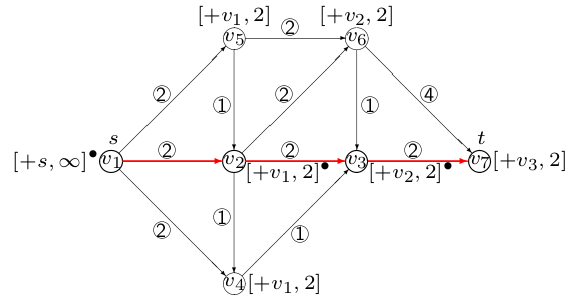
\includegraphics[width=0.8\textwidth]{images/cap7figura781.png}
  \caption{Prima iterazione}
  \label{cap7figura781}
\end{figure}

\item {\bf Incremento del flusso}: assegniamo a $\delta^*$ il valore
  $\delta(t)$ (cio\`e il valore di $\delta$ per il vertice $t$ (nel
  nostro caso $t = v_7$, $\delta(v_7) = 2$, $\delta^* = 2$), e
  prendiamo il vertice $t$ (cio\`e quello finale) e lo assegniamo alla
  variabile $x$. A questo punto inizia un ciclo su tutti i vertici
  {\em x} (partendo appunto dal vertice $t$) che termina soltanto nel
  momento in cui $x$ coincide con lo stato iniziale $s$:
  
  \begin{itemize}   
  \item {\bf Incremento del flusso - iterazione 1}: se l'etichetta del
    vertice $x$ \`e $[+y, \delta(x)]$ allora si pone al flusso
    sull'arco che va da $y$ a $x$ (quindi a $\xi_{yx}$) il valore
    $\xi_{yx}+\delta^*$. Dunque vediamolo applicato nella pratica: il
    nostro $t$ \`e $v_7$, la sua etichetta \`e $[+v_3,2]$. Assegniamo a
    $\xi_{37}$ il valore $\xi_{37} + \delta(7)$, quindi $0 + 2 =
    2$. Scriviamo tale valore sull'arco.  A questo punto assegniamo a
    $x$ il vertice $y$ e proseguiamo con le iterazioni dal momento che
    $x \neq s$. Se l'etichetta fosse stata $[-y, \delta(x)]$, allora
    avremmo posto $\xi_{xy}$ a $\xi_{xy}-\delta^*$.

  \item {\bf Incremento del flusso - iterazione 2}: proseguiamo
    all'indietro e individuiamo $\xi_{23} = 2$ e lo scriviamo
    sull'arco. Assegniamo a $x$ il vertice $y=2$, dunque continuiamo a
    iterare.

  \item {\bf Incremento del flusso - iterazione 3}: troviamo $\xi_{12}
    = 2$, lo mettiamo sull'arco e poniamo $x = y = v_1$. Essendo $v_1
    = s$ l'iterazione per l'incremento del flusso \`e finita. 
  \end{itemize} 

\item Cancelliamo tutte le etichette.

{\bf Prima iterazione del repeat (seconda iterazione del while)}:
dobbiamo ancora una volta etichettare $s$ con $[+s,+\infty]$ e
prendere un vertice etichettato ma non esplorato (che guarda caso
sar\`a $s$ essendo l'unico etichettato). Preso {\em s}, adesso
dobbiamo considerare gli archi uscenti per etichettare i relativi
vertici: i vertici di destinazione sono $v_2$, $v_4$ e $v_5$. Per il
primo non vale $\xi_{ij} < q_{ij}$ in quanto ora $\xi_{12} = 2$ e
$q_{12} = 2$, quindi prendiamo $v_4$ e $v_5$ e li etichettiamo come
abbiamo fatto in precedenza. Le etichette anche questa volta saranno:
$[+v_1, 2]$. Non abbiamo archi entranti in $s = v_1$, dunque non
dobbiamo fare altro; marchiamo $s = v_1$ come esplorato e passiamo al
prossimo vertice etichettato ma non esplorato.

\item {\bf Seconda iterazione del repeat (seconda iterazione del
  while)}: prendiamo il vertice $v_4$ e consideriamo gli archi uscenti
  e quelli entranti. Etichettiamo il vertice $v_3$ con $[+v_4,
    1]$. Questa volta etichettiamo $v_2$ in quanto \`e un arco
  entrante in $v_4$ e $\xi_{ij} > 0$. Lo etichettiamo con $[-v_3,
    1]$. Segnamo come esplorato il vertice $v_4$. 

\item Descrivere l'intero esempio sarebbe oltremodo lungo. L'algoritmo
  continua cos\`i fino a quando non si otterr\`a che $t$ non \`e
  etichettato alla fine del repeat. In questo caso si ottiene
  l'ottimo. Alla fine dell'algoritmo si attua un {\bf taglio} mettendo
  in $V_1$ i vertici etichettati ed in $V_2$ tutti gli altri.

\begin{figure}[h!]
  \centering
  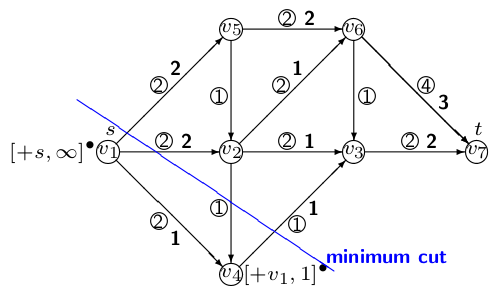
\includegraphics[width=0.8\textwidth]{images/cap7figura784.png}
  \caption{Risultato finale}
  \label{cap7figura784}
\end{figure}

\end{itemize}

Fine dell'esempio. $\blacktriangleleft$
\vspace{11pt}

\subsection{Altri problemi di flusso massimo}

Un altro problema di flusso massimo \`e quello in cui si vuole
trasmettere il massimo flusso possibile da un insieme {\em S} di
sorgenti ad un insieme di terminali {\em T} (con $S \cap T =
\emptyset$). Si pu\`o pensare come esempio ad un'azienda che produce
dei beni da pi\`u impianti e li deve distribuire a pi\`u depositi. Il
problema pu\`o essere ricondotto ad un MFP con l'aggiunta di due
vertici fittizi $v_s$ e $v_t$. Il primo funge da unica sorgente e
viene collegato a tutti i nodi di {\em S}, il secondo funge da unico
terminale e viene collegato a tutti i nodi di {\em T}. Ne deriva
dunque un nuovo grafo $G' = (V','A')$ in cui $V' \colonequals V \cup
\{ v_s, v_t\}$ e $A' \colonequals A \cup \{ (v_s, v_i) : v_i \in S\}
\cup \{ (v_j, v_t) : v_j \in T\}$. Se non vi sono altri vincoli, agli
archi fittizi aggiunti vengono assegnate capacit\`a infinite. Se
invece esistoo ad esempio limiti di produzione per gli impianti di
{\em S} o limiti di stoccaggio per gli impianti di {\em T}, questi
possono essere modellati assegnandoli come capacit\`a agli archi
fittizi corrispondenti.

Un'altra generalizzazione si presenta quando anche i
\underline{vertici} $v_i$ hanno una capacit\`a $p_i$ e il problema ha
il vincolo addizionale:

\begin{center}
\begin{equation}
\sum\limits_{v_k \in \Gamma^-(v_i)} \xi_{ki}\leq p_{ki}, \forall v_i
  \in V
\label{eq74}
\end{equation}
\end{center}

Anche questo problema pu\`o essere ricondotto ad un MFP come segue:

\begin{itemize}
\item si sdoppia ogni vertice $v_i$ in due vertici $v_i^+$ e $v_i^-$;
\item si collegano gli archi entranti in $v_i$ a $v_i^+$ e quelli
  uscenti a $v_i^-$;
\item si aggiunge un arco fittizio ($v_i^+, v_k^-$) con capacit\`a $p_i$.
\end{itemize}

Questo corrisponde a definire un nuovo grafo $G' = (V', A' \cup A'')$
con:

\begin{itemize}
\item $V' = \{ v_i^+ : v_i \in V\} \cup \{ v_i^- : v_i \in V\}$;
\item $(v_i^-, v_j^+) : (v_i,v_j) \in A$ con capacit\`a di $(v_i^-,
  v_j^+) = q_{ij}$;
\item $A'' = \{ (v_i^+,v_i^-) : v_i \in V\}$ con capacit\`a di
  $(v_i^+,v_i^-) = p_i$;
\end{itemize}

e si trova il flusso massimo da $s^+$ a $t^-$. Dato che tutto il
flusso entrante in un vertice $v_i^+$ deve fluire lungo l'arco
$(v_i^+, v_i^-)$ la capacit\`a dell'arco fittizio impone il rispetto
della condizione \ref{eq74}.

\begin{figure}[h!]
\centering
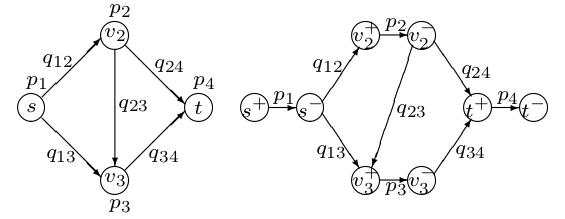
\includegraphics[width=0.8\textwidth]{images/cap7figura711.png}
\caption{Capacit\`a anche sui vertici}
\label{cap7figura711}
\end{figure}

\section{Modelli matematici}

Prima di vedere quali modelli matematici abbiamo per formalizzare in
altro modo i problemi sui grafi, introduciamo una nuova struttura
dati che prende il nome di {\bf matrice di incidenza}. Si tratta di
una matrice $A = [a_{ij}]$ con {\em n} righe (una per vertice) ed {\em
  m} colonne (una per arco) in cui al generico arco:

\begin{center}
  $a_{ik} = \begin{sistema}
    +1 \qquad  \text{se l'arco $a_k$ esce dal vertice $v_i$};\\
    -1 \qquad  \text{se l'arco $a_k$ entra nel vertice $v_i$};\\
    0 \qquad \text{altrimenti}.
  \end{sistema}$
\end{center}

Questa struttura spreca pi\`u memoria, ma risulta utile per la
formulazione di modelli.

\subsection{Cammini minimi e programmazione lineare}

Consideriamo il problema di trovare il cammino minimo da {\em s} a
{\em t}. Riformuliamolo come:

\begin{quote}
Trasmettere a costo minimo un flusso di materiale da {\em s} a {\em
  t}. Sia $\xi_k$ la quantit\`a di materiale che fluisce lungo l'arco
$a_k$ e interpretiamo $c_k$ (la lunghezza dell'arco $a_k$) come il
costo per ogni unit\`a di $\xi_k$ che fluisce lungo l'arco $a_k$.
\end{quote}

Il problema del cammino minimo da {\em s} a {\em t} \`e quindi
equivalente a quello di trovare un flusso unitario a costo minimo da
{\em s} a {\em t} in quanto abbiamo preso la lunghezza dell'arco come
costo per unit\`a di materiale da trasportare.

La legge di conservazione del flusso (osservando che ogni riga della
matrice contiene $-1$ e $+1$ per ogni arco entrante ed uscente) pu\`o
essere riscritta come:

\begin{center}
$a_i'\xi = 0 \quad \text{per} v_i \neq s,t$  
\end{center}

Cio\`e la differenza fra costo per unit\`a in entrata al nodo
dev'essere uguale al costo per unit\`a in uscita.

Possiamo dunque formulare un problema LP come:

\vspace{11pt}
\begin{center}
\begin{tabular}{l}
$(P) \min c'\xi$\\
$\qquad A\xi = \begin{bmatrix} 
+1 \quad \text{(s)}\\
-1 \quad \text{(t)}\\
0\\
\dots\\
0\\
\end{bmatrix}$\\
$\qquad\xi \geq 0$
\end{tabular}
\end{center}
\vspace{11pt}

mentre il suo duale \`e:

\vspace{11pt}
\begin{center}
\begin{tabular}{lp{3cm}l}
$(D) \max \pi_s - \pi_t$ & & $A_k$\\

$\begin{matrix}\qquad \pi' A \leq c' \\ \qquad \pi \gtreqless 0\end{matrix}$ & $\Leftrightarrow$ &
  $\begin{bmatrix}+1 \\ -1 \\ 0 \\ \dots \\ 0\end{bmatrix}$\\

$$ && \\
\end{tabular}
\end{center}
\vspace{11pt}

Notiamo come il problema primale abbia un vincolo per ogni vertice
(questo dipende dalla legge di conservazione del flusso) ed il
problema duale abbia un vincolo per ogni arco, della forma $\pi_i -
\pi_j \leq c_{ij}$ (dove $c_{ij}$ \`e il costo dell'arco $(v_i,v_j)$).

Si potrebbe sospettare che il modello non sia corretto in quanto la
soluzione $\xi$ potrebbe esser frazionaria, ossia prevedere una
separazione del flusso unitario in pi\`u flussi frazionari. In tal
caso per\`o tutti i cammini diversi che trasmettono frazioni di flusso
dovrebbero avere lo stesso costo unitario, per cui si potrebbe
convogliare tutto il flusso su uno qualunque di essi ottenendo una
soluzione intera equivalente. Pi\`u formalmente, vedremo nella
prossima sezione che una matrice di adiacenza \`e TUM.

\subsection{Una condizione sufficiente di unimodularit\`a}

{\bf Teorema:} una matrice {\em A} intera con $a_{ij} \in \{0, +1,
-1\} \forall i,j$ \`e TUM se:

\begin{enumerate}
\item nessuna colonna ha pi\`u di due elementi nulli e
\item le righe possono essere partizionate in due insiemi $I_1$ e
  $I_2$ tali che:

  \begin{itemize}
  \item se una colonna ha due elementi dello stesso segno, le loro
    righe sono in insiemi diversi;
  \item se una colonna ha due elementi di segno diverso, le loro righe
    sono nello stesso insieme.
  \end{itemize}

\end{enumerate}

\vspace{11pt}
$\square$ {\bf Dimostrazione}: dimostriamo la tesi per {\bf
  induzione}. Osserviamo che ogni sottomatrice quadrata di {\em A} di
ordine {\em 1} \`e unimodulare. Dimostriamo ora che se tutte le
sottomatrici di ordine {\em k-1} sono UM allora ogni matrice di ordine
{\em k} \`e UM. Sia {\em C} una sottomatrice di ordine {\em
  k}. Esistono tre casi possibili:

\begin{itemize}
\item {\em C} ha una colonna di soli zeri: quindi il determinante \`e
  0;
\item {\em C} ha una colonna con un solo elemento $c_{ij}$ non nullo:
  dunque il determinante vale $+1$ o $-1$ per il minore di
  $c_{ij}$. Poich\'e il minore \`e una sottomatrice di ordine $k-1$,
  dunque UM, consegue che {\em C} \`e UM;
\item {\em C} ha tutte colonne con due elementi non nulli: per ogni
  colonna {\em j} si ha allora $\sum_{i\in I_1} a_{ij} = \sum_{i\in
    I_2} a_{ij}$. Segue che la somma delle righe di $I_1$ meno la
  somma delle righe di $I_2$ vale 0. Questa \`e una combinazione
  lineare delle righe di {\em C}: se vale 0 allora il determinante di
  {\em C} \`e 0. $\blacksquare$
\end{itemize}
\vspace{11pt}

Le conseguenze del teorema sono tre e molto importanti:

\begin{enumerate}
\item La {\bf matrice di incidenza} di un grafo orientato \`e TUM;

\vspace{11pt}
$\square$ {\bf Dimostrazione}: Soddisfa l'ipotesi con $I_2 =
\emptyset$. $\blacksquare$
\vspace{11pt}

\item Il problema dei cammini minimi pu\`o essere risolto mediante
  programmazione lineare (e si pu\`o dimostrare che l'algoritmo di
  Dijkstra equivale ad una versione specializzata dell'algoritmo
  primale-duale).

\item la matrice dei vincoli del problema dell'assegnamento (AP) \`e
  TUM.
  
  \vspace{11pt} $\square$ {\bf Dimostrazione}: i vincoli illustrati
  nel modello visto nel capitolo 1 ai problemi di allocazione delle
  risorse modellano un LP in forma standard con $n^2$ variabili
  $x_{ij}$ e soddisfano l'ipotesi con $I_1 = \{1,\dots,n\}, I_2 = \{
  n+1,\dots,2n\}$.  $\blacksquare$
  \vspace{11pt}

  Si pu\`o quindi risolvere il rilassamento continuo dell'AP, in cui i
  vincoli $k_{ij} \in \{0,1\}$ sono sostituiti da $x_{ij} \geq 0$ (i
  vincoli $x_{ij} \leq 1$ sono ridondanti), con la certezza di
  ottenere una soluzione intera.

\end{enumerate}


\subsection{Flussi massimi e programmazione lineare}

Rappresentiamo il grafo di un {\em MFP} con una matrice di
incidenza. Indichiamo con $q_k$ la capacit\`a dell'arco $a_k$ e con
$\xi_k$ il flusso lungo l'arco $a_k\quad(k = 1,\dots,m)$. Un flusso di
valore {\em z} da {\em s} a {\em t} \`e allora espresso dal modello
lineare:

\vspace{11pt}
\begin{center}
\begin{tabular}{l}
$\xi \leq q$\\
$A\xi =
  \begin{sistema}
    +z\quad \text{riga s}\\
    -z\quad \text{riga t}\\
    0 \quad \text{righe $\neq$ s,t}
  \end{sistema}
$\\
$\xi \geq 0$\\
\end{tabular}
\end{center}
\vspace{11pt}

Introduciamo un vettore {\em d} di {\em n} costanti:

\begin{center}
  $d_i = 
  \begin{sistema}
    -1 \quad se i=s\\
    +1 \quad se i=t\\
    0 \quad se i \neq s,t.
  \end{sistema}
$  
\end{center}

La legge di conservazione del flusso:

\vspace{11pt}
\begin{center}
$\sum\limits_{v_j \in \Gamma^+ (v_i)}\xi_{ij} - \sum\limits_{v_k \in \Gamma^+ (v_i)}\xi_{ki} = \begin{sistema}
+z\phantom{aaa}v_i=s\\
-z\phantom{aaa}v_i=t, \forall v_i \in V\\
0\phantom{aaaa}altrimenti
\end{sistema}$
\end{center}
\vspace{11pt}

pu\`o essere riscritta come: $A\xi + dz = 0$. Una forma apparentemente
pi\`u debole \`e con il minore uguale. In realt\`a tale forma \`e
equivalente a quella data. Per ogni vertice $v_i \neq s, t$,
l'espressione $a_i'\xi$ esprime la differenza fra flusso uscente dal
vertice meno flusso entrante. Applicandola ai diversi vertici si ha:

\begin{enumerate}
\item {\bf riga {\em s}}: l'equazione $A\xi + dz \leq 0$ impone che il
  flusso uscente da {\em s} sia minore uguale di {\em z};
\item {\bf riga {\em t}}: l'equazione $A\xi + dz \leq 0$ impone che il
  flusso entrante in {\em t} sia maggiore o uguale a {\em z};
\item {\bf riga $i \neq s,t$}: l'equazione $A\xi + dz \leq 0$ impone
  che il flusso uscente da $v_i$ sia minore o uguale di quello
  entrante in $v_i$.
\end{enumerate}

Dalle ultime due risulta che il flusso uscente da $s$ \`e {\em z}. Da
ci\`o e dalla {\em 3} si ha che il flusso entrante in {\em t} \`e {\em
  z}. Da questa e {\em 3} consegue che il flusso uscente da $v_i$ \`e
uguale al flusso entrante in $v_i$ per ogni vertice che non sia {\em
  s} o {\em t}.

Il problema di flusso massimo pu\`o quindi essere modellato dall'LP in
{\em m+1} variabili:

\begin{center}
  
  \begin{tabular}{l}
    $(D)\quad \max z$\\
    $\qquad A\xi + dz \leq 0$\\
    $\qquad \xi \leq q$\\
    $\qquad -\xi \leq 0$\\
    $\qquad \xi, z \gtreqless 0$\\
  \end{tabular}

\end{center}

{\em D} pu\`o essere visto come il duale di un primale in forma
standard con vettore dei termini noti $b = (0,\dots,0,1) \geq 0$,
quindi idoneo all'applicazione dell'algoritmo primale-duale.

Il duale del primale ristretto \`e:

\begin{center}
  
  \begin{tabular}{l}
    $(DRP) \max z$\\
    $\qquad A\xi + dz \leq 0 \quad\text{ per tutte le righe}$\\
    $\qquad \xi \leq 0 \quad\text{ per tutte le righe corrispondenti a
      $\xi_{ij} = q_{ij}$}$\\
      $\qquad -\xi \leq 0 \quad\text{ per tutte le righe corrispondenti a
        $\xi_{ij} = 0$}$\\
      $\qquad A\xi \leq 1$\\
      $\qquad z \leq 1$\\
      $\qquad \xi, z \gtreqless 0$
  \end{tabular}

\end{center}

Il significato del DRP \`e: trovare un flusso unitario da {\em s} a
{\em t} che usi gli archi saturi all'indietro e gli archi a flusso
nullo in avanti. Proseguendo lo sviluppo formale \`e possibile
dimostrare che lo sviluppo di Ford-Fulkerson equivale ad una versione
specializzata dell'algoritmo primale-duale.


\section{Metodo CPM}

Un progetto complesso di qualunque tipo pu\`o essere visto come un
insieme di attivit\`a di diversa durata collegate da relazioni di
precedenza, ad esempio:

\begin{center}
{\em Y non pu\`o iniziare prima che X sia stata completata}.  
\end{center}

Tale vincolo viene espresso con la notazione $X \prec Y$.

\vspace{11pt}
$\blacktriangleright$ {\bf Esempio}: possiamo sintetizzare le fasi di
costruzione di una villetta con:

\begin{center}
\begin{tabular}{clcc}
{\bf Attivit\`a} & {\bf Descrizione} & {\bf Durata} & {\bf
  Predecessori} \\\hline
A & Scavo fondamenta & 4 & -\\
B & Costruzione struttura & 12 & A \\
C & Connessione tubature & 3 & A \\
D & Tubi acqua e riscaldamento & 6 & B \\
E & Posa cavi & 4 & B \\
F & Pavimenti e scarichi & 3 & B,C \\
G & Muri interni & 3 & D \\
H & Tetto e grondaie & 2 & E,F \\
I & Finitura interna & 5 & G \\
J & Pittura esterna & 3 & H \\
K & Pulizia finale & 1 & I,J \\
\hline  
\end{tabular}
\end{center}
$\blacktriangleleft$
\vspace{11pt}

Il progetto pu\`o essere ottimizzato trovando la sequenza di
esecuzione delle attivit\`a tale che la durata complessiva (che
chiamiamo {\bf makespan}) sia minima nel rispetto delle precedenze.

Esistono due tecniche principali: {\bf PERT} ({\em Program Evaluation
  and Review Technique}) e {\bf CPM} ({\em Critical Path Method}). Noi
ci concentreremo sul secondo. La differenza fra i due \`e che {\em
  CPM} presuppone dati deterministici, mentre l'altro aleatori.

\subsection{Fase 1: Grafo delle attivit\`a}

Modelliamo il progetto con un grafo orientato e pesato $G = (V,A)$ in
cui:

\begin{itemize}
\item gli archi $a_h = (v_i,v_j)$ rappresentano le attivit\`a;
\item i vertici rappresentano l'inizio o la fine delle attivit\`a;
\item il peso $d(v_i,v_j)$ \`e la durata dell'attivit\`a $(v_i,v_j)$;
\item il grafo rappresenta le relazioni di precedenza: $a_i \prec a_j$
  \`e imposto se il vertice finale di $a_i$ coincide col vertice
  iniziale di $a_j$ oppure se esiste un cammino contenente $a_i$ prima
  di $a_j$.
\end{itemize}

Non \`e possibile modellare il grafo usando soltanto le relazioni
esplicitamente formalizzate, ma \`e spesso necessario aggiungere delle
attivit\`a fittizie di durata nulla.

\vspace{11pt}
$\blacktriangleright$ {\bf Esempio}:

\begin{figure}[H]
  \centering
  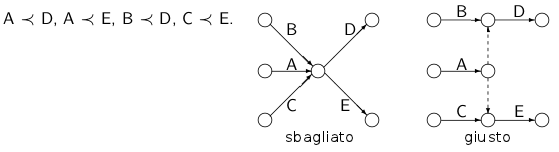
\includegraphics[width=\textwidth]{images/cap7fig713.png}
  \label{cap7figura713.png}
\end{figure}

A sx il modello sbagliato, a dx il modello corretto. Il modello di
sinistra \`e sbagliato in quanto con sol i5 archi si imporrebbero
precedenze non richieste, come quella fra B ed E e quella fra C e
D. $\blacktriangleleft$
\vspace{11pt}

Il grafo deve avere un solo vertice iniziale ed un solo vertice
terminale, entrambi con semigrado (rispettivamente entrante ed
uscente) nullo. Tali nodi modellano l'inizio e la fine del
progetto. Se il grafo non ha queste caratteristiche di suo, le si
modellano aggiungendo due vertici fittizi ed attivit\`a fittizie di
durata nulla.

Si otterr\`a sempre un grafo {\bf aciclico}, il contrario non avrebbe
senso logico. Il problema \`e quindi quello di determinare l'istante
di inizio di ogni attivit\`a in modo tale che il makespan sia minimo.

\subsection{Fase 2: Numerazione dei vertici}

Dobbiamo numerare i vertici in modo che per ogni arco $(v_i,v_j) \in
A$ si abbia $i < j$. Ci\`o in generale non \`e sempre possibile, ma lo
\`e per un grafo aciclico. Lo si fa tramite il seguente algoritmo che
ad ogni iterazione:

\begin{enumerate}
\item sceglie un vertice con semigrado entrante nullo;
\item gli attribuisce il primo numero disponibile;
\item elimina tutti gli archi uscenti dal vertice scelto.
\end{enumerate}

\vspace{11pt}
\begin{center}
  \begin{tabular}{||l||}
    \hline\hline
    {\bf procedure Number}:\\
    {\bf begin}\\
    \phantom{aa}se necessario, aggiungi a {\em G} i vertici fittizi
    $v_0$, $v_{n+1}$ e gli archi relativi;\\
    \phantom{aa}$B \colonequals A$ ({\bf comment:} copia di lavoro)\\
    \phantom{aa}$k \colonequals 0$;\\
    \phantom{aa}{\bf while} $k \leq n+1$ {\bf do}\\
    \phantom{aaaa}{\bf begin} ({\bf comment:} $\Gamma^-$ e $\Gamma^+$
    sono relativi al grafo $(V,B)$)\\
    \phantom{aaaaaa}scegli un vertice non numerato $v: \Gamma^-(v) = \emptyset$;\\
    \phantom{aaaaaa}attribuisci a {\em v} il numero $k$;
    \phantom{aaaaaa}$B \colonequals B \textbackslash \{(v,v_i) : v_i \in
    \Gamma^+(w)\};$\\
    \phantom{aaaaaa}$k \colonequals k+1$\\
    \phantom{aaaa}{\bf end}\\
    {\bf end.}\\
    \hline\hline
  \end{tabular}
\end{center}
\vspace{11pt}

Applicando quest'algoritmo all'esempio precedente otteniamo la
numerazione in figura \ref{cap7fig714}.

\subsection{Fase 3: Determinazione del makespan}

Con il seguente algoritmo determiniamo per ogni vertice $v_k$
l'istante minimo $TMIN_k$ in cui l'evento $v_k$ pu\`o accadere senza
violare le precedenze. Il {\bf makespan} \`e il valore di
$TMIN_{n+1}$. 

Dopo di ci\`o si determinano informazioni aggiuntive date per ogni
vertice $v_k$ dall'istante massimo $TMAX_k$ in cui l'evento $v_k$
pu\`o verificarsi senza ritardare il completamento del progetto.

In figura \ref{cap7fig714} troviamo anche la coppia $(TMIN_k,TMAX_k)$.

\vspace{11pt}
\begin{center}
  \begin{tabular}{||l||}
    \hline\hline
    {\bf procedure Critical Path:}\\
    {\bf begin}\\
    \phantom{aa}{\bf comment:} determina $TMIN_k$ per $k = 0,1,\dots,n+1;$\\
    \phantom{aa}$TMIN_0 \colonequals 0$;\\
    \phantom{aa}{\bf for} $k \colonequals 1$ {\bf to} $n+1$ {\bf do} $TMIN_k \colonequals
    \max_{i:(v_i,v_k) \in A} \{ TMIN_i + d(v_i,v_k)\}$;\\ 
    \\
    \phantom{aa}{\bf comment:} determina $TMAX_k$ per $k = n+1,n,\dots,0;$\\
    \phantom{aa}$TMAX_{n+1} \colonequals TMIN_{n+1}$;\\
    \phantom{aa}{\bf for} $k \colonequals n$ {\bf downto} 0 {\bf do }$TMAX_k \colonequals
    \min_{i:(v_k,v_i) \in A} \{ TMAX_i - d(v_k,v_i)\}$;\\ 
    {\bf end.}\\
    \hline\hline
  \end{tabular}
\end{center}
\vspace{11pt}

\begin{figure}[h!]
  \centering
  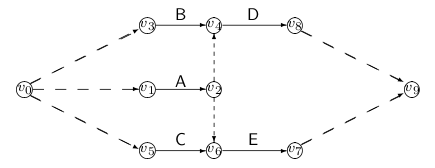
\includegraphics[width=\textwidth]{images/cap7fig714.png}
  \caption{Numerazione dei vertici e determinazione del makespan}
  \label{cap7fig714}
\end{figure}

\subsection{Fase 4: Definizione del piano esecutivo}

Per ogni attivit\`a $a_h = (v_i, v_j)$ si specificano le cosiddette
{\em informazioni caratteristiche}:

\begin{itemize}
\item {\bf Early Start Time}: $EST(a_h) = TMIN_i$;
\item {\bf Late Start Time}: $LST(a_h) = TMAX_j - d(v_i,v_j)$;
\item {\bf Float} (slittamento): $S(a_h) = LST(a_h) - EST(a_h)$.
\end{itemize}

Definiamo {\bf critica} ogni attivit\`a $a_h$ per la quale $LST(a_h) =
EST(a_h)$. Un cammino composto da ole attivit\`a critiche viene detto
{\bf cammino critico}.

\vspace{11pt}
$\blacktriangleright$ {\bf Esempio}: riprendendo l'esempio visto poco
fa possiamo realizzare la seguente tabella:

\vspace{11pt}
\begin{tabular}{cccccc}
  {\bf Attivit\`a} & {\em i} & {\em j} & $EST(v_i,v_j)$ &
  $LST(v_i,v_j)$ & $S(v_i,v_j)$ \\\hline
A & 1 & 2 & 0 & 0 & 0 \\
B & 3 & 4 & 0 & 2 & 2 \\
C & 5 & 6 & 0 & 2 & 2 \\
D & 4 & 8 & 7 & 7 & 0 \\
E & 6 & 7 & 8 & 10 & 2 \\
\end{tabular}
\vspace{11pt}

Le attivit\`a A e D sono critiche. Il cammino
$\{v_0,v_1,v_2,v_4,v_8,v_9 \}$ \`e critico perch\'e come possiamo
vedere ogni attivit\`a ha $EST$ e $LST$ uguale.

Di solito si utilizza il {\bf diagramma di Gantt} per rappresentare la
soluzione al problema. Qui di seguito vediamo il diagramma relativo al
nostro caso:

\begin{figure}[H]
  \centering
  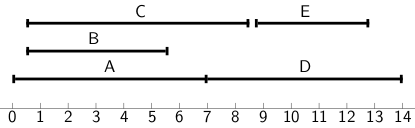
\includegraphics[width=0.9\textwidth]{images/cap7figura715.png}
  \caption{Diagramma di Gantt}
  \label{cap7figura715}
\end{figure}

Fine dell'esempio. $\blacktriangleleft$
\vspace{11pt}

\vspace{11pt} $\blacktriangleright$ {\bf Esempio}: riprendendo il caso
della villetta possiamo vedere in figura il grafo corrispondente e la
soluzione.

\begin{figure}[H]
  \centering
  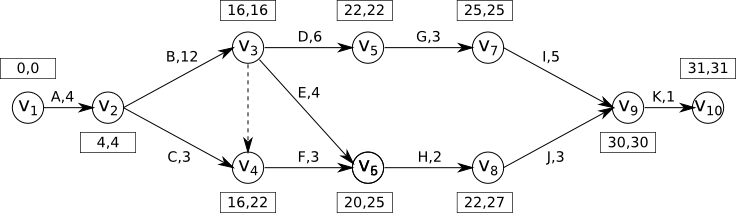
\includegraphics[width=\textwidth]{images/cap7figura716.png}
  \caption{Esempio di determinazione del makespan}
  \label{cap7figura716}
\end{figure}

In questo caso esistevano gi\`a due attivit\`a {\em A} e {\em K}
rispettivamente senza predecessori e senza successori, dunque non \`e
stato necessario aggiungere due vertici $v_0$ e
$v_{n+1}$. $\blacktriangleleft$
\vspace{11pt}

\section{Circuiti Hamiltoniani}

Dato un grafo orientato e non pesato $G=(V,A)$, un {\bf circuito
  hamiltoniano} ({\em HC}) \`e un circuito che visita tutti i vertici
di {\em V} una ed una sola volta.

Per stabilire se un grafo possiede un {\em HC} si utilizza un
{\em algoritmo enumerativo} basato su un albero
decisionale. L'algoritmo base effettua una ricerca {\em depth-first}
estendendo progressivamente un cammino $S = \{v_1,\dots,v_l\}$
finch\'e:

\begin{itemize}
\item nessun vertice pu\`o essere aggiunto a {\em S} e tuttavia non
  sono stati coperti tutti i vertici (quindi $|S|<n$); in questo caso
  si effettua un {\em backtracking};
\item i vertici sono stati coperti tutti, dunque $|S| = n$ e quindi
  $S$ \`e un cammino hamiltoniano (se $(v_l,v_1) \in A$).
\end{itemize}

\vspace{11pt}
$\blacktriangleright$ {\bf Esempio}: vediamo il grafo 

\begin{figure}[H]
  \centering
  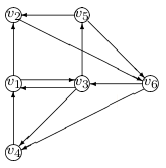
\includegraphics[width=0.3\textwidth]{images/cap7hamilton1.png}
  \caption{Un grafo}
  \label{cap7hamilton1}
\end{figure}

e cerchiamo di trovare un circuito hamiltoniano. Iniziamo dal nodo
$v_1$ e mettiamo nella radice dell'albero il valore 0 in quanto \`e il
passo iniziale. Adesso dobbiamo compiere il passo 1 e lo facciamo
muovendoci sull'arco $(v_1,v_2)$. Dal nodo $v_2$ possiamo muoverci
solo verso $v_6$ dunque il prossimo arco che esploriamo \`e
$(v_2,v_6)$. Da $v_6$ possiamo raggiungere $v_3$ e $v_4$, quindi
iniziamo esplorando il primo dei due. Da $v_3$ possiamo raggiungere
soltanto $v_4$ e $v_5$. Anche in questo caso iniziamo esplorando il
primo dei due. Arrivati in $v_4$ l'unico passo possibile \`e tornare
in $v_1$, ma ci\`o non va bene in quanto il nodo $v_1$ \`e gi\`a
esplorato e il nodo $v_5$ non l'abbiamo visitato. 

Dobbiamo quindi fare il backtracking. Il primo punto di scelta che
troviamo tornando indietro \`e al passo che abbiamo numerato con 3. Il
passo in cui abbiamo scelto $(v_3,v_4)$ in luogo di
$(v_3,v_5)$. Effettuiamo questa volta la scelta contraria. Arriviamo
nel vertice $v_5$, ma anche in questo caso non abbiamo la
possibilit\`a di esplorare nodi nuovi, ma solo nodi gi\`a
visitati. Occorre un altro backtracking. Il punto di scelta aperto
immediatamente precedente \`e al punto 2 dell'albero. Da $v_6$ ci
eravamo mossi verso $v_3$, ora invece ci muoviamo verso $v_4$. Questa
scelta non ci permette di procedere oltre, dunque ritorniamo ancora
pi\`u indietro. Il nodo su cui fare backtracking ora \`e proprio il
nodo radice. Da $v_1$ prendiamo l'arco $(v_1,v_3)$. Dal vertice $v_3$
abbiamo a disposizione una scelta fra $(v_3,v_4)$ e $(v_3,v_5)$. Il
primo arco non porta a nulla, prendiamo il secondo e arriviamo nel
vertice $v_5$. Da questo nodo scegliamo l'arco $(v_5, v_2)$. Dal
vertice $v_2$ possiamo solo muoverci in $v_6$, da $v_6$ solo in $v_4$
in quanto $v_3$ \`e gi\`a stato visitato con questo cammino e infine
notiamo che, non solo abbiamo esplorato tutti i vertici, ma esiste
anche l'arco che porta dall'ultimo vertice visitato ($v_4$) al vertice
iniziale $v_1$, dunque abbiamo trovato un circuito
hamiltoniano. Possiamo procedere oltre, vedendo se ne esistono altri,
ma in questo caso la ricerca non produce risultati.

L'albero risultante lo troviamo in figura \ref{cap7hamilton2}.

\begin{figure}[H]
  \centering
  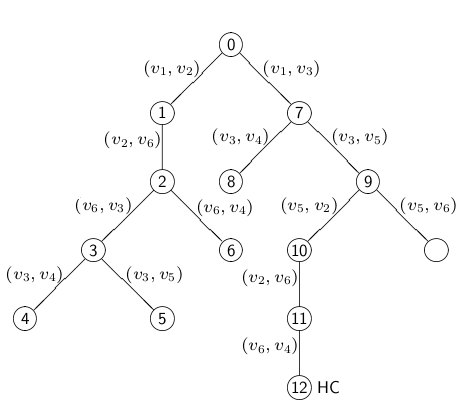
\includegraphics[width=0.7\textwidth]{images/cap7hamilton2.png}
  \caption{L'albero decisionale}
  \label{cap7hamilton2}
\end{figure}

$\blacktriangleleft$
\vspace{11pt}

Nei problemi di ricerca di HC non essendoci costi non \`e possibile
applicare i bound per accelerare la ricerca. \`E possibile per\`o
utilizzare altre tecniche per uccidere nodi dell'albero
decisionale. Ad esempio quando aggiungiamo l'arco $(v_l, v_s)$ ad {\em
  S} possiamo eliminare da $A$ (l'insieme degli archi):

\begin{itemize}
\item gli archi $(v_l,v_i)$ con $i\neq s$;
\item gli archi $(v_j,v_s)$ con $j\neq l$.
\end{itemize}

Tali archi andranno poi riaggiunti quando si fa il backtracking su
$(v_l,v_s)$.

Consideriamo l'operazione di branching sul cammino attuale $S =
\{v_1,\dots,v_l\}$. Valgono le seguenti {\bf regole}:

\begin{itemize}
\item se $\exists (v_l,v_i) \in A, v_i \not\in S: |\Gamma^-(v_i)| = 1$
  (cio\`e se esiste un arco che porta dal vertice $v_l$, che \`e
  l'ultimo raggiunto, al vertice $v_i$ non ancora visitato e tale che
  in $v_i$ ci sia solo un arco entrante) allora si deve generare solo
  il figlio corrispondente a $(v_l,v_i)$ (cio\`e si deve visitare ora
  il nodo $v_i$ altrimenti non lo si potrebbe raggiungere in seguito);

\item se $\exists (v_l, v_j), (v_l, v_k)$ con le caratteristiche
  dell'arco $(v_l,v_i)$ della regola precedente si pu\`o effettuare un
  backtracking;

\item se $\exists (v_l,v_i), (v_k,v_i) \in A, v_i, v_k \not\in S:
  |\Gamma^+(v_k) = 1|$ (cio\`e se esistono due archi che portano da
  due vertici $v_l$ e $v_k$ non visitati in $v_i$ e da $v_k$ non vi
  sono altri archi uscenti se non quello che porta in $v_i$), allora
  non si deve generare il figlio corrispondente a $(v_l,v_i)$, ma si
  deve generare l'altro perch\'e altrimenti una volta giunti in $v_k$
  non si potrebbe proseguire oltre.
\end{itemize}

\vspace{11pt}
$\blacktriangleright$ {\bf Esempio}: rivediamo il grafo precedente ed
applichiamo le regole appena citate. Il risultato \`e mostrato in
figura \ref{cap7hamilton3}.

Il passo 1 ci porta nel vertice $v_2$, ma questo \`e raggiungibile
anche da $v_5$ e se notiamo bene il nodo $v_5$ pu\`o andare solo in
$v_2$ dunque una volta arrivati in $v_5$ non avremmo uscita. Ecco
dunque che possiamo applicare la regola 3 e tagliare questo ramo.

Passiamo ora a vedere come applichiamo la regola 1. Arrivati nel passo
2, nel vertice $v_3$ vediamo che da questo nodo possiamo visitare
$v_4$ e $v_5$ e vediamo che il vertice $v_5$ non lo potremmo
raggiungere in seguito in quanto l'unico arco entrante in questo nodo
passa proprio da $v_3$ dunque applichiamo la regola 1 e tagliamo
l'altro ramo.

A questo punto l'esplorazione continua e vediamo che arriviamo ad
ottenere un circuito Hamiltoniano in meno passi.

\begin{figure}[H]
  \centering
  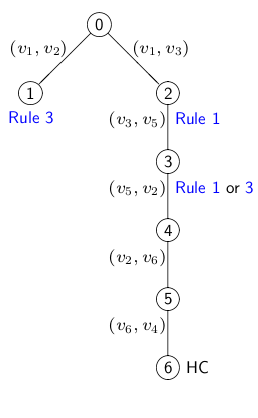
\includegraphics[width=0.4\textwidth]{images/cap7hamilton3.png}
  \caption{L'algoritmo migliorato per HC}
  \label{cap7hamilton3}
\end{figure}

$\blacktriangleleft$
\vspace{11pt}

\section{Traveling Salesman Problem}

Il {\bf problema del commesso viaggiatore} ({\em TSP}) \`e una
generalizzazione del problema HC. Consiste, dato un grafo pesato
(orientato o meno) nel trovare il circuito hamiltoniano di costo
minimo.

Si assumer\`a che la matrice dei costi sia completa, con $c_{ij} = +
\infty$ per eventuali spigoli $(v_i,v_j)$ non presenti nel grafo dato.

Considerando un'applicazione magari relativa ad una mappa stradale,
pu\`o capitare che l'arco (la strada) che collega due vertici
(citt\`a) $v_i$ e $v_j$ abbia un costo maggiore di un percorso che
collega gli stessi vertici passando per un terzo vertice $v_k$. In
questa situazione chiaramente preferiremmo passare per la terza
citt\`a pur di risparmiare tempo o chilometri. Questo non \`e
ammissibile per un HC, dunque si impone che valga la {\bf condizione
  di triangolarit\`a}:

\begin{center}
$c_{ij} \leq c_{ik} + c_{kj} \quad (i,j,k=1,\dots,n)$  
\end{center}

Se il grafo non dovesse rispettare questa condizione di
triangolarit\`a, si disegna un arco diretto da $v_i$ a $v_j$ con il
peso del percorso che passa da $v_k$. Questo \`e quello che si chiama
{\bf rilassamento AP}.

I modelli matematici e gli algoritmi sono diversi a seconda che si
tratti di un grafo orientato ({\em Asymmetric TSP, ATSP}) o meno ({\em
  Symmetric TSP, STSP}):

\begin{itemize}
  
\item {\bf ATSP}: un classico modello \`e:

  \vspace{11pt}
  \begin{center}
  \begin{tabular}{l}
    $\min \sum\limits_{i=1}^n\sum\limits_{j=1}^nc_{ij}x_{ij}$\\
    $\quad\sum\limits_{i=1}^n x_{ij} = 1 \qquad (j=1,\dots,n)$\\
    $\quad\sum\limits_{j=1}^n x_{ij} = 1 \qquad (i=1,\dots,n)$\\
    $\quad\sum\limits_{i \in S, j \not\in S}^n x_{ij} \geq 1 \qquad \forall
    S\quad\subset V, S \neq \emptyset$\\
  \end{tabular}
  \end{center}
  \vspace{11pt}

  dove: $x_{ij}$ vale 1 se l'arco $(v_i,v_j)$ \`e in soluzione, 0
  altrimenti.

  La prima sommatoria dei vincoli, quella su {\em i}, impone
  che esattamente un arco entri in ciascun vertice. La seconda impone
  che esattamente un arco esca da ciascun vertice. Il terzo vincolo
  serve invece per eliminare dalle soluzioni i circuiti parziali.

  Mentre le prime due equazioni comportano $2n$ vincoli, la terza ne
  comporta un numero esponenziale che rende molto difficile la
  soluzione del problema mediante il modello.

\item {\bf STSP}: Identifichiamo ogni spigolo con un numero intero
  {\em e} e gli associamo una variabile $x_e$ che valga 1 se lo
  spigolo \`e in soluzione, 0 altrimenti. Per un vertice $v_i$
  indichiamo con $\delta(i) = \{ (v_i,v_j) : v_j \in V\}$ l'insieme di
  spigoli adiacenti. Per un insieme di vertici $S \subset V$ con $(S
  \neq \emptyset)$ indichiamo con $E(S) = \{ (v_i,v_j) : v_i \in S,
  v_j \in S \}$ l'insieme degli spigoli interni ad {\em S}. Si ha
  allora il modello:

  \vspace{11pt}
  \begin{center}
  \begin{tabular}{l}
    $\min \sum\limits_{e\in E} c_ex_e$\\
    $\quad\sum\limits_{e \in \delta(i)} x_e = 2 \qquad (i=1,\dots,n)$\\
    $\quad\sum\limits_{e \in E(S)} x_e \leq |S|-1 \forall S \subset V,
    S \neq \emptyset$\\
    $x_e \in \{0,1\} \forall e \in E$\\
  \end{tabular}
  \end{center}
  \vspace{11pt}

  La prima equazione dei vincoli impone che ogni vertice abbia
  esattamente due spigoli adiacenti, la seconda impone che nessun
  sottoinsieme di vertici contenga un circuito parziale. Anche in
  questo caso l'ultima equazione impone vincoli in numero
  esponenziale.

\end{itemize}

Per risolvere i {\em TSP} vi sono molte tecniche: branch and bound,
piani di taglio, branch and cut, programmazione dinamica. 

Risolvendo con il branch and bound classico, ad ogni nodo si risolve
il rilassamento che si ottiene eliminando le equazioni che abbiamo
detto introdurre un numero esponenziale di vincoli. Se ci sono
circuiti parziali, i nodi figli vengono generati imponendo condizioni
che li impediscano. Nel caso peggiore questo algoritmo pu\`o
degenerare in una enumerazione completa. 

\section{Problemi di Vehicle Routing}

I problemi industriali di distribuzione di merci sono di norma pi\`u
complessi del TSP in quanto possono prevedere pi\`u di un veicolo e
pi\`u di un deposito, nonch\'e insiemi di vincoli specifici legati al
problema da risolvere, al contratto di lavoro delle persone impiegate,
agli orari di apertura delle strutture interessate, ecc\dots

Questi problemi hanno grande rilevaza pratica, in quanto si calcola
che il trasporto incide di una percentuale compresa fra il 10 ed il
25\% sul costo finale dei beni. Utilizzare tecniche di ottimizzazione
pu\`o portare ad una riduzione dei costi di trasporto compresa fra il
5\% ed il 20\%.

Possiamo dunque definire una classe di problemi che va sotto il nome
di {\bf Vehicle Routing Problem} ({\em VRP}):

\begin{quote}
Determinare un insieme di percorsi, ciascuno effettuato da un veicolo
che parte e ritorna al deposito di competenza, nel rispetto di
specifici vincoli operativi, minimizzando il costo complessivo del
trasporto.
\end{quote}

Faremo adesso una panoramica delle varie classi di problemi di Vehicle
Routing. In generale si usano grafi orientati se i problemi sono
relativi ad una rete stradale urbana (dove quindi possono esservi
anche dei sensi unici), oppure non orientati per reti
extra-urbane. Noi faremo riferimento a questo secondo caso e
considereremo un grafo non orientato con costi $c_{ij}$ associati agli
spigoli $(v_i,v_j)$. Inoltre faremo l'assunzione che vi sia un solo
deposito dal momento che l'estensione al caso con pi\`u depositi \`e
immediata.

\subsection{Capacitated Vehicle Routing Problem ({\em CVRP})}

Questo \`e il problema di base. Nel grafo avremo:

\begin{itemize}
\item un vertice $v_0$ che rappresenta l'unico deposito;
\item i vertici $v_i\quad(i=1,\dots,n)$ che rappresentano i clienti;
\item il cliente $i$ richiede merci di peso totale
  $d_i\quad(i=1,\dots,n)$;
\item ogni cliente deve essere visitato da un solo veicolo;
\item sono disponibili $K$ veicoli con capacit\`a $C_k,\quad
  (k=1,\dots,K)$.
\end{itemize}

Il problema consiste nel determinare un insieme di non pi\`u di {\em
  K} circuiti (e i rispettivi vincoli) che servano tutti i clienti, in
modo che il peso totale trasportato da ciascun veicolo non superi la
corrispondente capacit\`a ed il costo complessivo sia minimo.

\subsection{Distance-constrained Vehicle Routing}

Il problema \`e un'estensione del precedente realizzata con l'aggiunta
di un vincolo:

\begin{itemize}
\item ad ogni spigolo \`e associato un tempo di percorrenza $t_{ij}$;
\item ad ogni veicolo $k$ \`e anche imposto un massimo tempo di
  viaggio $T_k\quad (k=1,\dots,K)$.
\end{itemize}


\subsection{Vehicle Routing with Time Windows}

Anche questo \`e un'estensione del {\em CVRP} con un vincolo
aggiuntivo da rispettare:

\begin{itemize}
\item ad ogni spigolo \`e anche associato un tempo di percorrenza
  $t_{ij}$;
\item ad ogni cliente {\em i} sono associati tre valori $s_i$, $a_i$ e
  $b_i$, che rappresentano:

  \begin{itemize}
  \item $s_i$: il tempo necessario per servire il cliente {\em i};
  \item $[a_i,b_i]$: l'intervallo di tempo in cui deve iniziare il
    servizio del cliente {\em i}.
  \end{itemize}

\end{itemize}

I tempi $s_i$ devono essere sommati ai tempi di percorrenza
$t_{ij}$, nell'ordine opportuno. In certi casi i tempi di percorrenza
coincidono con i costi $c_{ij}$.

\subsection{Vehicle Routing with backhauls}

Anche questo \`e un'estensione del {\em CVRP} con due vincoli
aggiuntivi. I clienti sono posizionati in due sottoinsiemi:

\begin{itemize}
\item {\em linehaul customers}: ai quali i veicoli consegnano merci;
\item {\em backhaul customers}: dai quali i veicoli ritirano merci.
\end{itemize}

Ogni veicolo deve visitare i linehaul customers assegnatigli prima di
tutti i backhaul customers assegnatigli. Inoltre per ogni veicolo {\em
  k} si deve avere $\max\{(peso totale consegnato),(peso totale
ritirato)\} \leq C_k$.

\subsection{Vehicle Routing with pickup and delivery}

Al problema {\em CVRP} si aggiungono i seguenti vincoli. Ad ogni
cliente {\em i} sono associati due valori:

\begin{itemize}
\item $d_i$: quantit\`a di merci da consegnare al cliente;
\item $p_i$: quantit\`a di merci da prelevare dal cliente.
\end{itemize}

Quando il veicolo arriva presso il cliente, effettua prima le
operazioni di scarico e poi quelle di carico. Per ogni veicolo {\em k}
il peso totale presente in qualunque momento non deve superare $C_k$.

\subsection{Vehicle Routing with loading constraints}

Al {\em CVRP} viene aggiunto il seguente vincolo:

\begin{itemize}
\item ad ogni cliente {\em i} \`e associato l'elenco dei pacchi
  richiesti con le rispettive dimensioni (altezza, larghezza,
  profondit\`a);
\item per ogni veicolo sono note le dimensioni dell'area di carico.
\end{itemize}

La soluzione deve prevedere per ogni veicolo la definizione della
sistemazione ({\em packing}) nell'area di carico dei pacchi.

\end{document}
